\documentclass[a4j, 12pt]{jsarticle}
\usepackage[dvipdfmx]{graphicx}
\usepackage[top = 35truemm, bottom = 45truemm, left = 30truemm, right = 30truemm]{geometry}
\usepackage{fancyhdr}
\usepackage{comment}
\usepackage{titlesec}
\usepackage{here}
\usepackage{hhline}
\usepackage{url}
\usepackage{multirow}
\usepackage{algpseudocode,algorithm}

\titleformat*{\section}{\Huge\bfseries}
\makeatletter

\def\@thesis{2020年度 修士論文}
\def\id#1{\def\@id{#1}}
\def\department#1{\def\@department{#1}}
\def\teacher#1{\def\@teacher{#1}}
\def\research#1{\def\@research{#1}}
\renewcommand{\thesection}{第\arabic{section} 章}
% 図・表番号の設定
\renewcommand{\theequation}{\arabic{section}.\arabic{equation}}
\renewcommand{\thefigure}{\arabic{section}.\arabic{figure}}
\renewcommand{\thetable}{\arabic{section}.\arabic{table}}
\@addtoreset{equation}{section}
\@addtoreset{figure}{section}
\@addtoreset{table}{section}

\def\@maketitle{
\begin{center}
\vspace*{10mm}
{\LARGE \underline{\@thesis} \par}
\vspace{15mm}
{\Huge\bf \@title \par} % 論文のタイトル部分
\vspace{20mm}
{\Large \@date\par} % 提出年月日部分
\vspace{15mm}
{\Large 指導教員: \@teacher 教授\par}
{\Large 研究指導名: \@research 研究\par}
\vspace{15mm}
{\Large \@department \par} % 所属部分
\vspace{5mm}
{\Large 学籍番号: \@id \par} % 学籍番号部分
\vspace{5mm}
{\Large \@author}% 氏名
\newpage
\end{center}
\par\vskip 1.5em
}

\makeatother
\title{ウェブページの重要領域の視覚化に関する研究}
\date{2021年1月25日(月)提出}
\teacher{深澤良彰}
\research{ソフトウェア開発工学}
\department{
  早稲田大学大学院 基幹理工学研究科\\
  情報理工・情報通信専攻 深澤研究室
}
\id{5119F009-4}
\author{稲垣 有哉}

\pagestyle{fancyplain}

\begin{document}
\pagestyle{empty}
\maketitle

% 目次出力箇所
\pagenumbering{roman}
\setcounter{page}{1}
\pagestyle{plain}
\setcounter{tocdepth}{3} %目次をどこまで表示するか
\tableofcontents

\newpage
\pagenumbering{arabic}
\setcounter{page}{1} %ページのスタート番号
\pagestyle{fancy}
\lhead{2020年度 修士論文}
\rhead{早稲田大学大学院基幹理工学研究科 深澤研究室}

% 本文

% 第1章 はじめに
\renewcommand{\baselinestretch}{1.5} % 行間の倍率指定
\section{はじめに}\label{sec:introduction}
\renewcommand{\baselinestretch}{1} % 行間の倍率指定

% 既存の研究・顕著性マップではどこが重要、目立っているのかがわかりづらいという問題点がある。

% インターネットの普及率の推移とウェブマーケティング市場の増加について記述
\par 近年インターネット普及により我々の身の周りでは数えきれないほど多くのウェブサイトが開発されている。NetCraftのWeb Server Surveyによると図\ref{fig-num_websites}に示すように2018年12月時点で世界中に15億を超えるウェブページが存在し、2008年から約10倍まで増加している\cite{webserver_survey}。さらにITRによると日本国内のウェブマーケティング市場は2016年度に売り上げ金額が16億円で前年比142.9\%増の急速な伸びとなり今後も引き続き市場拡大すると予想している\cite{itr_webmarket}。この為スマートフォンやタブレット端末が普及した今、ウェブページは誰もが閲覧するもので極めて重要性が高いと言える。

\begin{figure}[H]
    \centering
    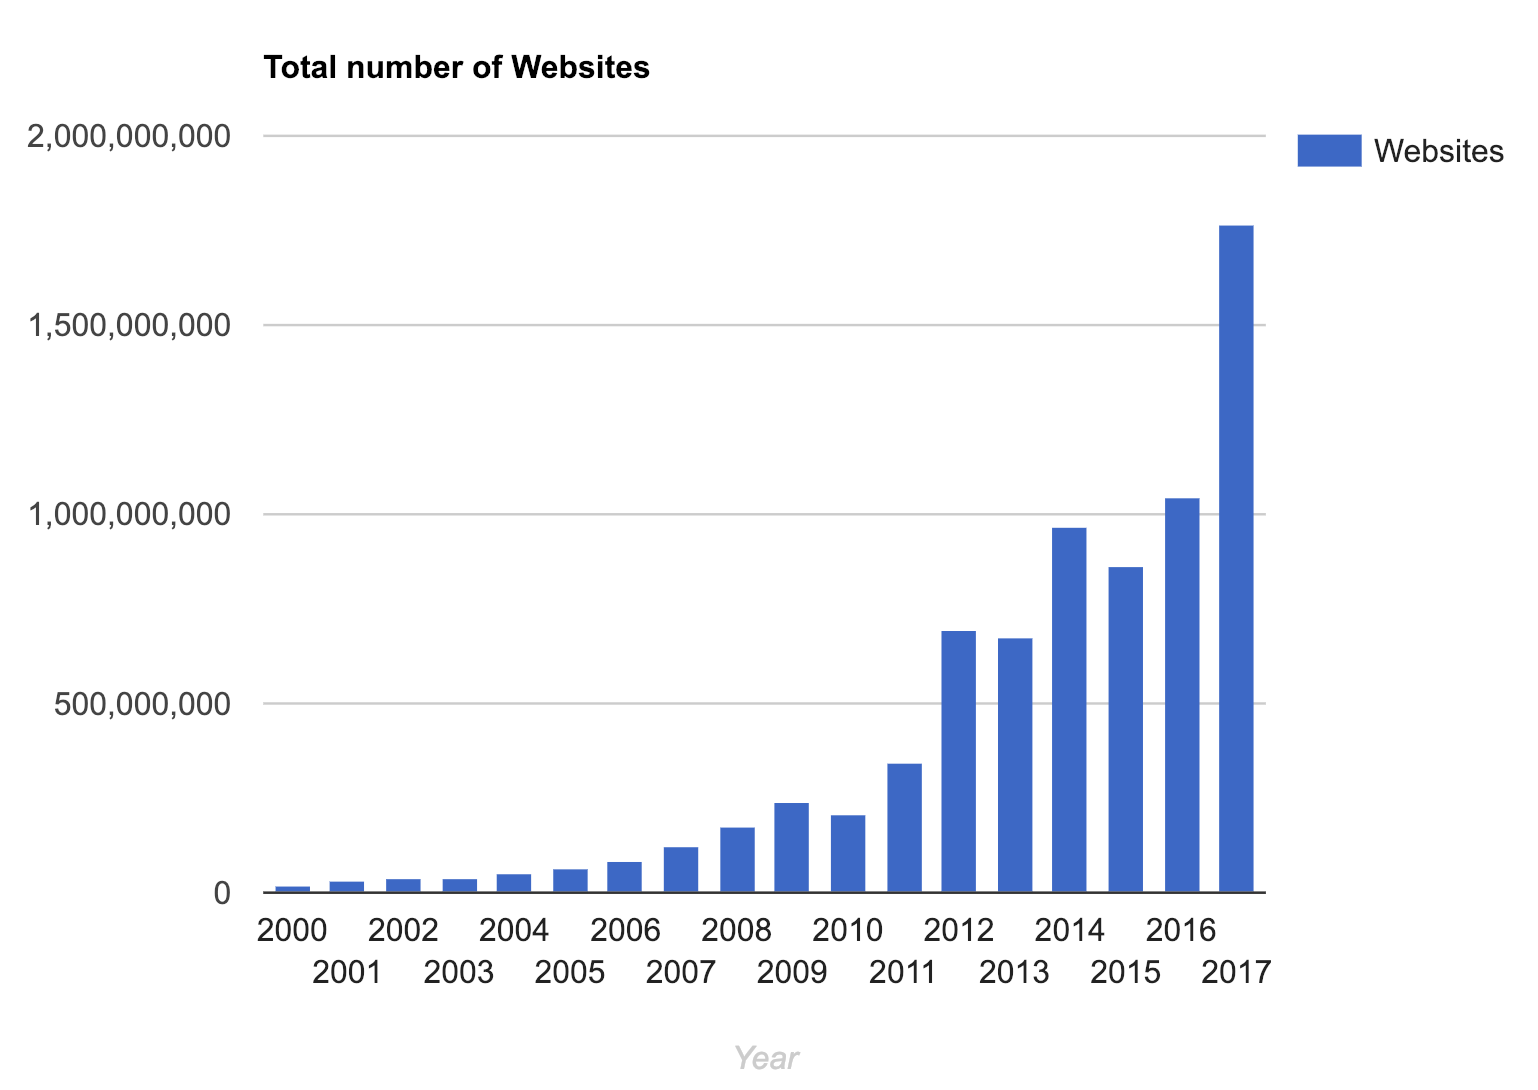
\includegraphics[width=8cm]{figures/number-of-websites.png}
    \caption{全世界のウェブサイトの数の推移\cite{internetlivestats}}
    \label{fig-num_websites}
\end{figure}


% ユーザビリティが低いサイトは離脱率が高いという問題がある
\par ウェブサイトを開発する時にデザイナーはユーザーに興味を持ってもらえるようなデザインかつ目的の要素に簡単に到達可能となるようにレイアウトを設計する。しかしながら、実際にはデザインが良くても目的の要素を見つけづらいと感じたり使いづらいと感じるユーザビリティが低いウェブページは数多くある。ユーザーはユーザビリティが低いウェブページから離れやすい傾向があり、結果的にサービスの質の低下に繋がってしまう。これはデザイナーの意思がしっかりとデザインに反映されず、デザイナーが見て欲しい情報とユーザーが実際に見ている情報にズレがあることが原因の一つである。

% 問題の解決方法・既存顕著性マップの見づらさ
\par このような問題を未然に防ぐための一つの手法として、人の注視の引きつけやすさを示す顕著性マップをデザイナーに開発段階で示すことでユーザーが注目する可能性が高い領域を事前に知ることが効果的であると考える。風景や人の顔などの自然画像の顕著性マップ生成モデルに関する研究は多数存在するが、ウェブページに特化した顕著性マップの生成モデルについての研究はほとんど存在しない。また、顕著性マップを見ただけでは具体的にウェブページのどの要素が目立っているのか分かりづらい。

% 提案手法の概略
\par そこで本研究では、開発段階でウェブページの構造と顕著性マップを組み合わせることで要素単位で顕著性を計算することによるウェブページの重要領域の視覚化手法を提案する。私はデザイナーがウェブページの開発・設計時にどの部分にユーザーの注目が集まるかを予想して解析対象のウェブページ上に視覚的に描画することでウェブページの設計の効率化に繋がると考えている。また、ページ中のどこに注目が集まりやすいかを予測しそれに合わせて注目してほしい情報を注目されやすいようにデザイナーが配置することで、その情報にユーザーが注目しやすくなり効率的なユーザーの獲得につながるのではないかと考えられる。
\par さらに、要素単位で顕著度のランキングを生成して特に顕著度が高い重要領域を1つの画像に集約したウェブページの集約図を提示する事によるページ内容理解支援手法を提案する。ユーザーが注目する可能性が高い顕著性が高い領域にはウェブページの重要な内容が含まれる事が多い為、該当領域を集約した図を提示する事でウェブページの内容の理解支援に繋がるのではないかと考えられる。

% 論文の構成
\par 本論文は、本章を含め全8章で構成される。第2章では本研究で使用するウェブページの構造について紹介し、第3章では本研究の背景となる視覚的顕著性と顕著性マップの知識について紹介する。第4章では本研究と関連する研究について述べ、第5章では本研究の特徴について述べる。第6章では本研究の詳細について述べ、第7章で本研究の評価について述べる。最後に第8章おわりにで、全体の内容をまとめ今後の課題を述べる。
% 第2章 ウェブページの構造
\newpage
% \section{ウェブページの構造}\label{sec:webpage}
% \par 本章では、本研究で使用するウェブページの構造とその取得方法について説明する。
% \subsection{HTML}
% \subsubsection{HTMLとは}
% \par 近年PHPやRubyなど様々なプログラミング言語によりウェブページやウェブアプリケーションは開発されているが、最終的にはHTML(Hyper Text Markup Language)と呼ばれるマークアップ言語を動的に出力することでウェブブラウザ上にウェブページを表示している。つまり、HTMLを分析することでウェブページの構造が分かるということだ。
% \par HTMLには様々なバージョンが存在するが、W3Techsによると現在主流であるHTML5は76.0\%のシェアを誇る\cite{html_share}。本論文でHTML5を取り扱うことにした。

% \subsubsection{HTMLの代表的なタグ}
% \par HTMLでは決められたタグと呼ばれるマークアップを使用してソースコードが記述される。HTML5には数多くのタグが存在するが、その中でも代表的なタグを表\ref{table:SpeedOfLight}に示す。

% \begin{table}[h]
%     \caption{HTMLの代表的なタグ\cite{mozilla_html}}
%     \label{table:SpeedOfLight}
%     \centering
%      \begin{tabular}{clll}
%       \hline
%       タグ & 意味 \\
%       \hline \hline
%       \textless html\textgreater & HTML文書において基点となるトップレベル要素 \\
%       \textless head\textgreater & 文書に関する全般的な情報を内包する要素 \\
%       \textless title\textgreater & ブラウザに表示される文書の題名 \\
%       \textless body\textgreater & HTML文書のコンテンツを示す要素 \\
%       \textless div\textgreater & フローコンテンツの汎用コンテナー \\
%       \textless img\textgreater & 文書に画像を埋め込むための置換要素 \\
%       \textless a\textgreater & ハイパーリンク \\
%       \textless h1\textgreater & 文書中の見出しを示す為の要素 \\
%       \textless p\textgreater & テキストの段落を表す \\
%       \textless span\textgreater & 記述コンテンツの汎用的な行内コンテナー \\
%       \hline
%     \end{tabular}
% \end{table}

\renewcommand{\baselinestretch}{1.5} % 行間の倍率指定
\section{ウェブページの構造}\label{sec:scraping}
\renewcommand{\baselinestretch}{1} % 行間の倍率指定
\par 近年PHPやRubyなど様々なプログラミング言語によりウェブページやウェブアプリケーションは開発されているが、最終的にはHTML(Hyper Text Markup Language)と呼ばれるマークアップ言語\cite{mozilla_html}を動的に出力することでウェブブラウザ上にウェブページを表示している。つまり、HTMLを分析することでウェブページの構造が分かるということだ。それらの構造を解析する事で様々な情報を取得する方法としてウェブスクレイピング技術がある。
\subsection{ウェブスクレイピングとは}
\par サーバーサイドのプログラムを使用することで外部サーバーにアクセスしてウェブサイト上から必要な情報を取得することをウェブスクレイピングという\cite{ntt_scraping}。似たような技術としてAPIが存在するがAPIはサービス提供者側が技術者向けに情報提供する機能のことで、ウェブスクレイピングとは異なる。通常はウェブページのタイトルや株価などの可変数値を取得する目的で使用されることが多いが、本研究ではスクリーンショットの取得やウェブページの構造解析の為にHTMLと各タグ要素の位置情報を取得する為に使用する。

\subsection{ライブラリ}
\par ウェブスクレイピングを簡単に出来るように汎用性のあるプログラムを再利用可能なように集めたライブラリが数多く存在する。ここでは本研究で使用したSelenium WebDriver\cite{selenium}とBeautiful Soup\cite{beautifulsoup}の2つのライブラリを説明する。

\begin{itemize}
    \item Selenium WebDriver
    \par ~~Selenium WebDriverはウェブアプリケーションの自動テストツールとして開発され、ウェブブラウザの拡張機能を使用する事でJavaやPython等のプログラムでブラウザの自動操作を行う事が可能である。本研究では、PythonでSelenium WebDriverを使用する事でスクリーンショットやHTMLの取得のほか画像等の要素の位置とサイズを取得する目的で使用した。 \\

    \item Beautiful Soup
    \par ~~Beautiful SoupはSelenium WebDriverとは異なりPython用のライブラリで、取得したHTMLからタグを抽出したり必要な情報を取得したりする事が可能である。本研究では、Selenium WebDriverを用いて取得したHTMLを解析しやすいように加工する目的でBeautiful Soupを使用した。 \\
\end{itemize}

% 第3章 関連研究
\newpage
%自分の研究との比較が可能なものだけ関連研究に載せる
\renewcommand{\baselinestretch}{1.5}
\section{関連研究}
\renewcommand{\baselinestretch}{1}
\par 近年画像解析技術の進歩により風景などの自然画像の顕著性マップ生成モデルに関する研究は多くされているが、ウェブページに特化した顕著性マップ生成モデルに関する研究はほとんど存在しない。

\subsection{自然画像の顕著性マップ生成モデル}\label{subsec:related-01}
\par 自然画像の顕著性を計算するモデルは昔から研究されて様々なモデルが存在する。中でも基本的な顕著性マップ生成モデルとしてItti-Kochらの顕著性モデル\cite{itti1998model}は広く知られている。このモデルでは、人間の目の視覚認識と同様に色・輝度・方向のそれぞれの視覚特徴を抽出した後に重み付けして足し合わせることにより顕著性マップを生成するモデルである。図\ref{fig_itti-kochi}に計算モデルの構造を示す。このモデルは視覚的顕著性に関連性のある数多くの研究で利用されている。

\begin{figure}[H]
    \centering
    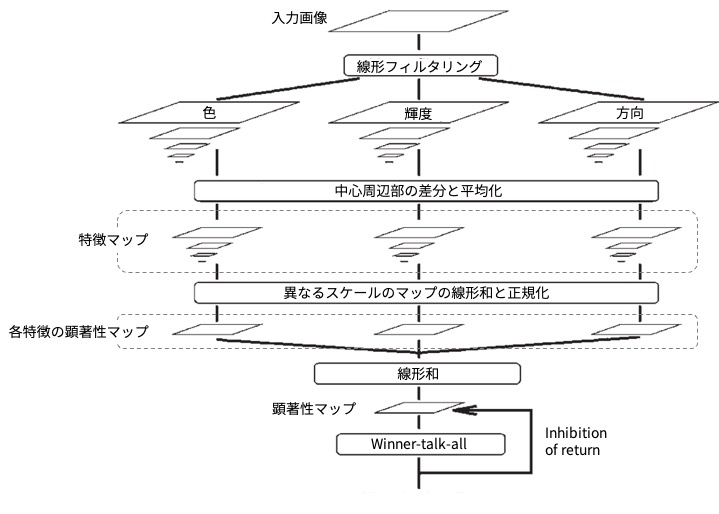
\includegraphics[width=8.5cm]{figures/itti-kochi-model.jpg}
    \caption{Itti-Kochらによる顕著性計算モデルの構造\cite{itti1998model}\label{subsec:related-01}}
    \label{fig_itti-kochi}
\end{figure}

\par 近年の技術の進歩により大規模なデータセットからトレーニングされたディープラーニング手法を活用したモデルが多く研究されている。PanらによるSalNet\cite{pan2016shallow}では顕著度を最初から予測するために独自の畳み込みニューラルネットワーク(CNN)を学習して構築された。また、学習済みの畳み込みニューラルネットワークを使用する事でJiangらによるSALICON\cite{jiang2015salicon}やCorniaらによるML-NET\cite{Cornia_2018}やKummererらによるDeep Gaze 2\cite{kummerer2016deepgaze}などの自然画像向けの顕著性マップ生成モデルを構築されている。KummererらはMITの顕著性マップのベンチマークであるmit300\cite{mit-saliency-benchmark}のAUCの評価において他のモデルと比較して最も良い精度であることを明らかにした。

\par しかしながら、いずれの研究においても風景などの自然画像をベースに学習されたモデルであるためウェブページのように特有の要素があるものは正確に判断することが難しい。


\subsection{グラフィックデザインの顕著性マップ生成モデル}\label{subsec:related-02}
\par 自然画像だけでなくグラフィックデザインに特化した顕著性マップ生成モデルも存在する。Bylinskiiらはポスターなどのグラッフィックデザインとテキストや表が含まれるデータの2種類に分け、それぞれのデータセットを異なる形式で収集してニューラルネットワークモデルを構築することで既存のものと比較して精度の高いグラフィックデザインの顕著性マップを生成可能であることを示している\cite{bylinskii2017learning}。
\par しかしながら、この手法ではウェブページの構造などを考慮していないため顕著度を正確に判断することが難しい。


\subsection{ウェブページの構造分析に関する研究}\label{subsec:related-03}
\par 野中らはウェブページの構造を分割するVIPSアルゴリズムの問題点を指摘して、オリジナルの手法でウェブページの構造解析とタグの情報から内容を分析する事で手法掲載箇所の抜き出しを行う手法の提案を行い、従来の手法と比較して有効な結果を得られることを示した\cite{weko_66695_1}。また、Caiらは視覚的表現にもとづいてコンテンツ間の関係を識別する事でウェブコンテンツの構造を抽出する手法を提案し、従来のDOMベースの手法と比較して良い結果が出たことを明らかにしている\cite{cai2003extracting}。
\par しかし、これらの手法では抽出したレイアウト構造から重要度が高い領域を検出することは出来ない。


\subsection{ウェブページの顕著性マップ生成モデル}\label{subsec:related-04}
\par さらにウェブページに特化した顕著性マップ生成モデルも僅かに存在する。人間の注意は大きく分けて色や輝度や方向などの低レベル特徴が主のボトムアップ要因と過去の経験に基づく記憶依存や知識駆動などのトップダウン要因の2つに分けられる。
\par Shenらは従来のボトムアップ要因の顕著性モデルにトップダウン要因を組合せる事で既存のものと比較して精度の高いウェブページの顕著性マップを生成可能であることを示している\cite{shen2014webpage}。彼らは左上の領域が比較的注目されやすい傾向にあるという位置バイアスや人の顔写真に注目が集まりやすいフェイスバイアスをトップダウン要因としてボトムアップ要因とマルチカーネル学習を使用して全ての特徴を統合する事で顕著性マップを生成した。Guptaらはモバイルデバイスとデスクトップデバイスの違いに着目し、スマートフォンの前面カメラを使用して視線を認識し視線データを学習する事で要素レベルでのモバイルUI向け顕著性マップ生成モデルを生成した\cite{Gupta_2018}。また、Zhengらは様々なタスク条件下でユーザーが注目する領域を予測する顕著性予測モデルを考案した。彼らはタスク固有の顕著性予測モデルとタスクなしの自由閲覧条件下での顕著性予測モデルを組み合わせることでタスク駆動型の顕著性マップ生成モデルを構築している\cite{Zheng_task-driven}。

\par しかしながら、いずれの研究においても最終的な出力は顕著領域をヒートマップ形式で表現した顕著性マップのみである。精度が高い顕著性マップを出力しても一目ではどの領域が注目されやすいのか正確に判断する事は難しい。

% 第4章 本研究の特徴
\newpage
\renewcommand{\baselinestretch}{1.5}
\section{本研究の特徴}
\renewcommand{\baselinestretch}{1}
\par 本研究の特徴は既存の顕著性マップ生成モデルとウェブページの構造を組合せる事で、ウェブページのレイアウトを考慮して要素単位での顕著度を正確に予測するということである。要素単位の顕著度を正確に予測するためにウェブページ閲覧時の視線データセットを作成した。計算した顕著度を用いて、ピクセル単位ではなく要素単位での顕著性を視覚化して顕著領域マップの生成を行う。また、要素の顕著度ランキングを計算して顕著度が高い領域をトリミングすることで重要度の高い領域を視覚化する集約図の生成を行う。

\subsection{視線データセットの作成}
\par 人間の注視はボトムアップ要因とトップダウン要因の二種類の特徴を組み合わせて処理を行う。ボトムアップ要因とは輝度特性や色特性や方向特性などで、周囲の刺激と顕著に異なる場合に注意が引き付けられる。一方でトップダウン要因とは事前知識などがある際にそれらに基づいて能動的にバイアスがかかり注意が引き付けられることを示す。風景などの自然画像と比較してウェブページには写真やテキストやロゴなどの固有の要素が多数存在していてこれらが正確な顕著性の予測を困難にしている。Shenら\cite{shen2014webpage}の人間の視線を測定するアイトラッカーを用いてウェブページの顕著性を測定した実験によると、図\ref{fig_shen-experience}に示すようにテキスト中心と画像中心とテキスト画像が混合した全てのウェブページにおいて人は左上の領域と中心付近に目線が行く傾向が判明した。ウェブページの左上から中央にかけての領域に注目が集まるの現象はf-biasと言う名で一般的に知られており、このようにバイアスを考慮して正確な顕著性を予測するためにユーザーがウェブページを閲覧する際の視線データが必要となる。しかしながら、ウェブ上に公開されている視線のデータセットはほとんど存在しておらず、近年のモダンデザインに対応しているものは存在しないためオリジナルデータセットを作成する。

\begin{figure}[H]
  \centering
  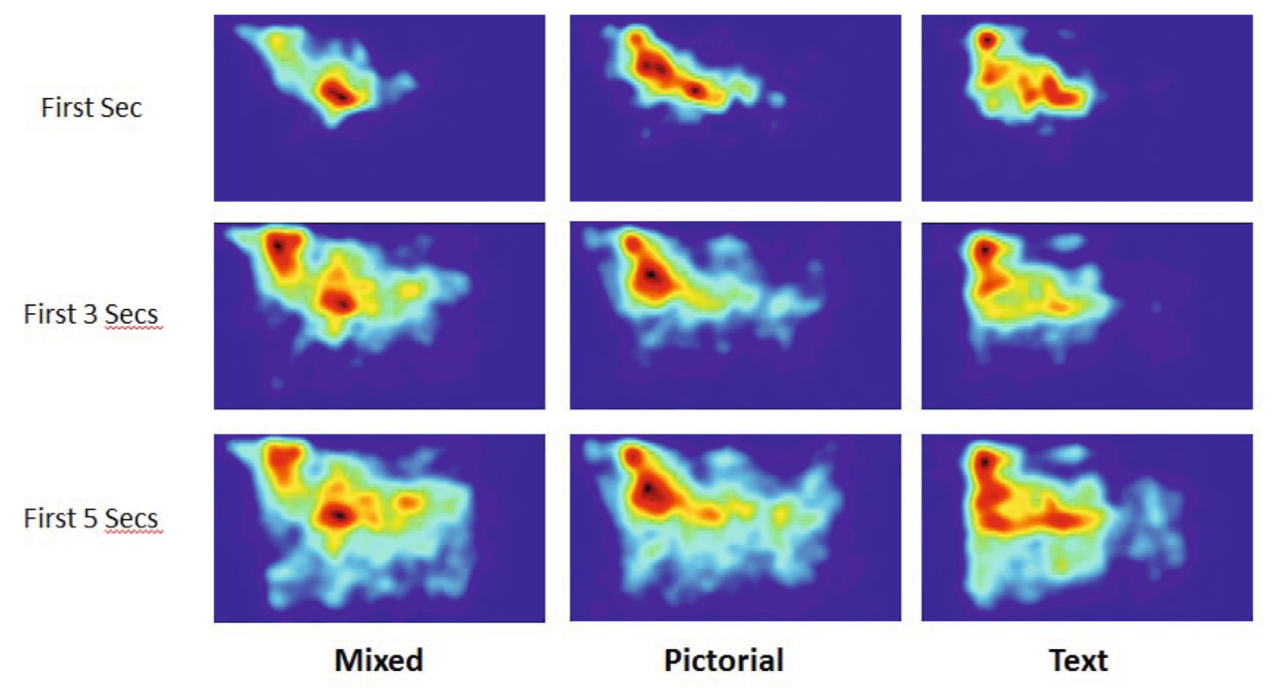
\includegraphics[width=8cm]{figures/shen-bias.png}
  \caption{Shenらのウェブページのヒートマップ生成実験結果\cite{shen2014webpage}}
  \label{fig_shen-experience}
\end{figure}

\subsection{要素単位での顕著性マップの生成}
\par 通常の顕著性マップではグレースケールで顕著性を表現するが、これだけではどの領域が重要度が高いであろうというざっくりとした予想しか行う事ができない。ウェブページを閲覧する際に人は、画像やタイトルやリンクなどタグ単位の要素で重要度を判断する事が多い。そこで本研究では要素単位の顕著性を計算してランキング付けをする事で、正確にどの要素の顕著性が高いのか判断できるウェブページに特化した要素単位の顕著領域マップを生成する事が効果的だと考えた。図\ref{fig_comparesaliency}に早稲田大学ウェブサイトトップページ(2018年12月時点)\cite{waseda_top}のスクリーンショットを入力した時に生成される既存の顕著性マップと提案手法の顕著領域マップの比較を示す。なお、提案手法の顕著領域マップ上の緑色の枠線は特に顕著度が高い重要領域10箇所を表している。

\begin{figure}[H]
    \centering
    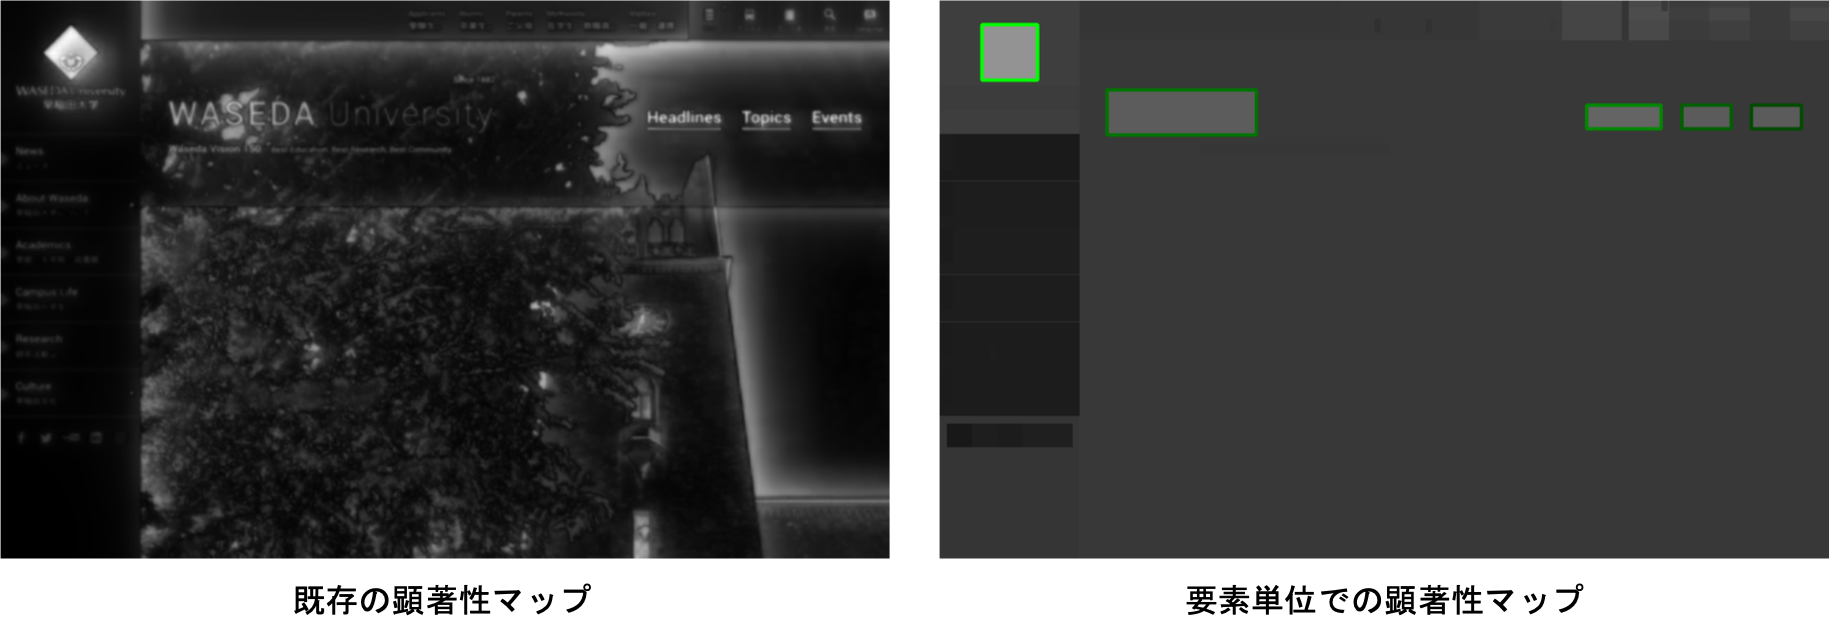
\includegraphics[width=12cm]{figures/example-originalsaliencymap.png}
    \caption{既存の顕著性マップと要素単位での顕著性マップとの比較}
    \label{fig_comparesaliency}
\end{figure}

\subsection{重要領域の視覚化}
\par ウェブページの顕著領域にはウェブページの重要な内容が含まれる事が多い。既存の研究では精度の高い顕著性マップの生成を行う事で研究が完結している事がほとんどである。しかしながら、要素ごとの顕著性を計算する事で作成した顕著度ランキングを元に重要領域ををタイル状に並べて一つの画像にまとめる事でウェブページの内容を簡単に把握可能な集約図を生成出来ると考えた。これにより、ネットユーザーが初見のウェブページにアクセスした際の内容把握の時間短縮に繋がる可能性がある。図\ref{fig_imoortanceregion}に早稲田大学ウェブサイトトップページ(2018年12月時点)\cite{waseda_top}の重要領域を集約した集約図を示す。

\begin{figure}[H]
    \centering
    
\includegraphics[width=8cm]{figures/example-importanceregion.png}
    \caption{生成された集約図の例}
    \label{fig_imoortanceregion}
\end{figure}

% 第6章 本研究の詳細
\newpage
\renewcommand{\baselinestretch}{1.5}
\section{本研究の詳細}
\renewcommand{\baselinestretch}{1}

\par デザイナーが検証するウェブページのURLを入力すると該当ページの顕著性マップとページの構造を組み合わせることにより顕著度が高い領域を要素単位で分析して顕著領域マップを出力する手法を提案する。また、一般ユーザー向けに特に顕著度が高い領域を纏めて描写した集約図を出力する手法を提案する。本手法の構造図を図\ref{fig_ourmodel}に示す。

\begin{figure}[H]
    \centering
    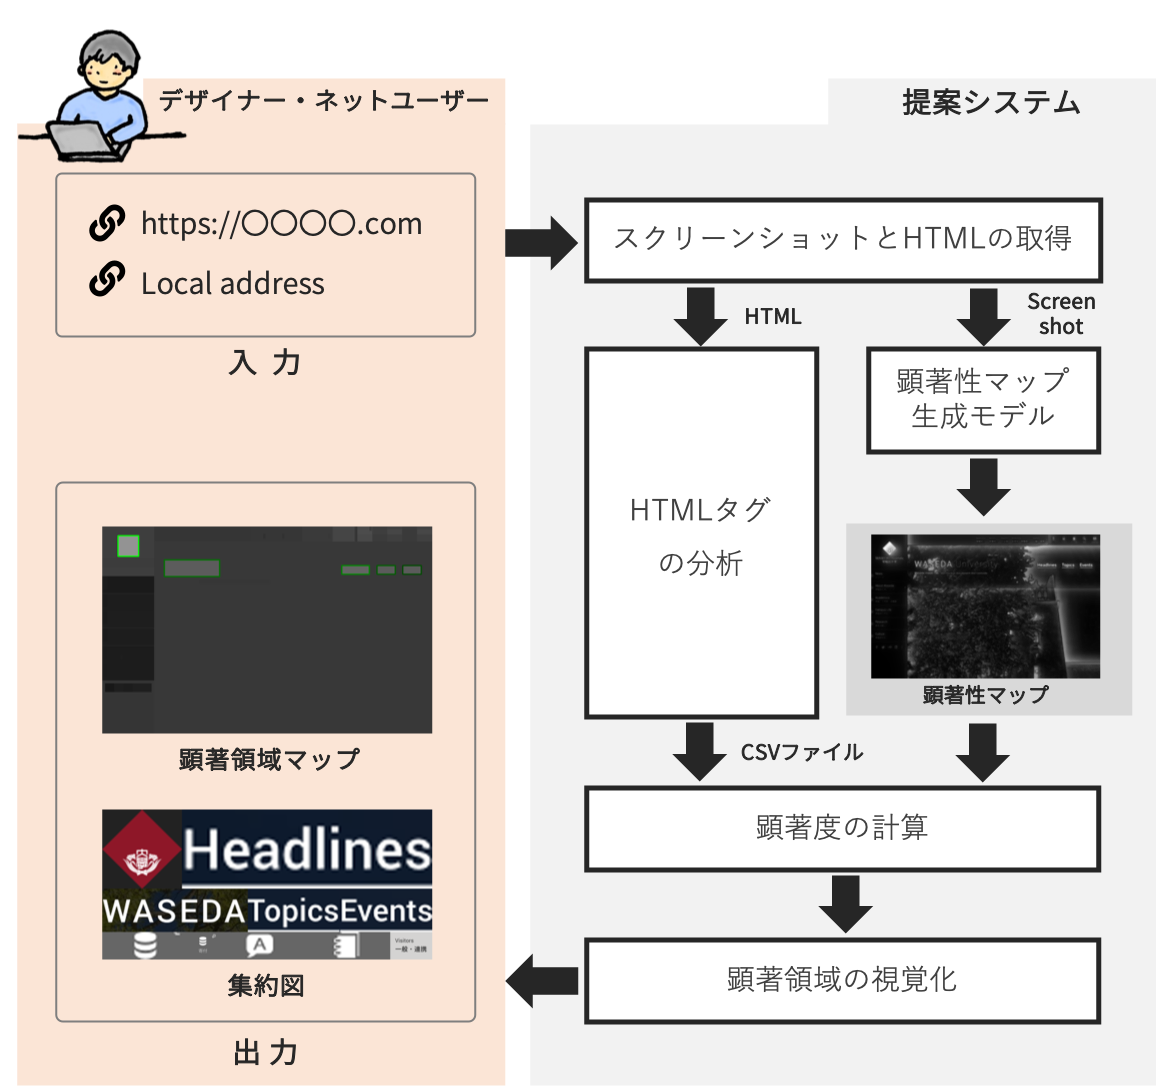
\includegraphics[width=9cm]{figures/model.png}
    \caption{モデルの図}
    \label{fig_ourmodel}
\end{figure}

\par 本手法の手順は以下の通りである。
\par(1) HTMLの取得と顕著性マップの生成
\par(2) HTMLの解析によるタグの分析と位置の取得
\par(3) 顕著度の計算
\par(4) 顕著領域の視覚化\\

\par なお、本研究ではウェブスクレイピング技術としてSelenium WebDriverとBeautiful Soupを使用するが別のスクレイピング技術を使用しても実装は可能である。また、スクリーンショットを取得するブラウザとしてFirefoxを使用するがChromeなど別のブラウザでも実装可能である。

\subsection{HTMLの取得と顕著性マップの生成}\label{subsec:system01}
% ウェブスクレイピング技術を使用してスクショを取得する方法とHTMLの取得方法の記述
% スクショのグレースケール変換方法・サイズの圧縮
%  Selenium WebdriverでFirefoxの立ち上げ・該当URLへの移動
%  Selenium WebdriverでHTMLの取得
%  Beautiful Soupを用いてHTMLの整形
%  Selenium Webdriverでスクショの取得・保存
%  顕著性マップの生成
%  OpenCVを用いて顕著性マップの二値化  
%  OpenCVを用いてスクショと顕著性マップの指定サイズへの圧縮

\par 本システムではまず、入力されたURL情報を元に\ref{sec:scraping}で説明したウェブスクレイピング技術を用いてスクリーンショットとHTMLを取得する。また、取得したスクリーンショットを用いて顕著性マップを生成する。デザイナーが開発段階で簡単に使用可能な様に入力するURLは、ネットワーク上に存在するウェブページだけでなくローカル環境のURLにも対応させている。HTMLの取得と顕著性マップの生成の流れを図\ref{fig_system01}に示す。

\begin{figure}[H]
    \centering
    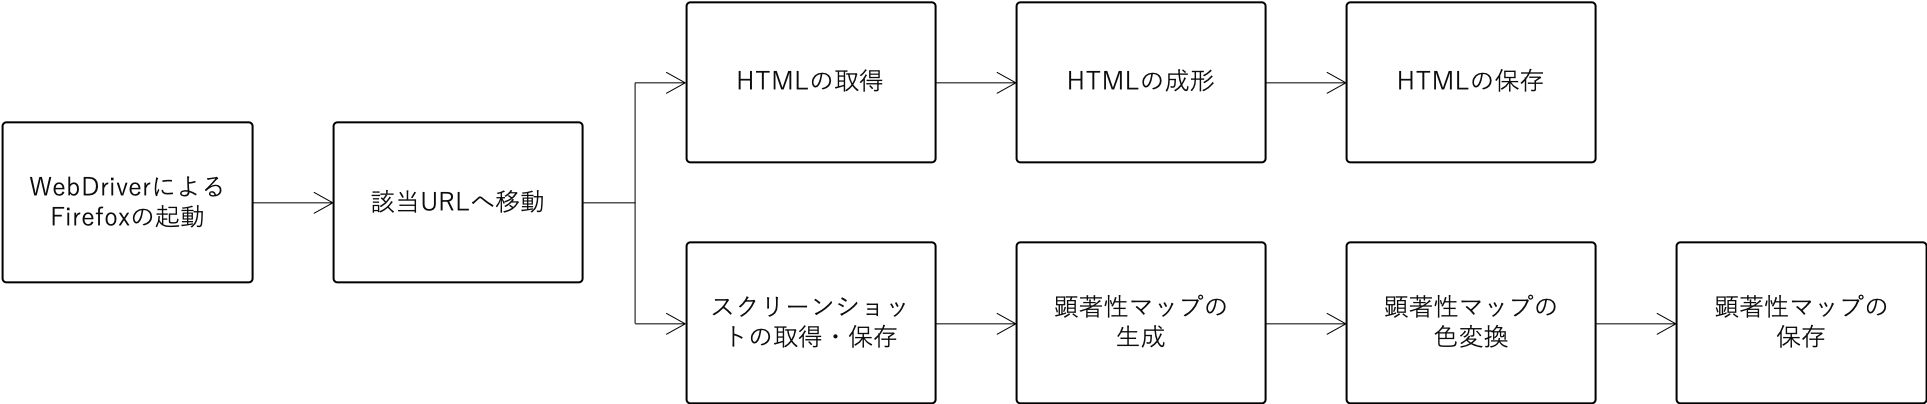
\includegraphics[width=12cm]{figures/system01.png}
    \caption{HTMLの取得と顕著性マップの生成の流れ}
    \label{fig_system01}
\end{figure}

\par まず始めに、Selenium WebDriverを用いてFirefoxを起動し、ブラウザのウィンドウサイズを一般的なパソコンで閲覧する条件に近い横1280px縦900pxに設定する。次に入力されたURLにアクセスを行い、ウェブページの読み込みが完了したらHTMLの取得を行う。取得したHTMLはインデントなどが乱れた状態である為、Selenium WebDriverと同じくウェブスクレイピング技術のライブラリであるBeautiful Soup\cite{beautifulsoup}を使用して扱いやすい状態に整形を行った後に保存する。

\par 次にウェブページのスクリーンショットを取得する。取得するスクリーンショットは、重要度が高いコンテンツはウェブページの最上部に存在する可能性が高いという考えから、ウェブページにアクセスした時点で閲覧可能な最上部の横1280px縦900pxとした。さらに、取得したスクリーンショットから顕著性マップを生成する。顕著性マップの生成には第\ref{subsec:itti-kochi}節で説明したItti-Kochらの顕著性マップ生成モデルを使用した。本来であれば、ウェブページに最適化された精度の高いモデルを使用すべきであるが現時点では技術的に難しいと判断し扱いやすいモデルを使用することにした。ここで顕著性マップ生成モデルにより出力される顕著性マップはRGBの3色チャンネルで出力されるが、後の処理で明度を使用するために単色チャンネルで表されるグレースケール画像に変換して保存する。取得される顕著性マップの例が図\ref{fig_example-saliencymap}(右)である。


\subsection{HTMLの解析によるタグの分析と位置の取得}\label{subsec:system02}
% 各タグの存在確認と位置情報の取得方法の記述
%  CSVの準備(ヘッダーの準備)
%  Selenium Webdriverで各タグの位置情報の取得(xpathとサイズ取得方法の説明を入れる)

\par ここでは第\ref{subsec:system01}節で取得したHTMLの解析を行いウェブページ上の要素の位置情報とそのサイズを取得する。HTMLの解析によるタグの分析と位置の取得の流れを図\ref{fig_system02}に示す。

\begin{figure}[H]
    \centering
    
\includegraphics[width=12cm]{figures/system02.png}
    \caption{HTMLの解析によるタグの分析と位置の取得の流れ}
    \label{fig_system02}
\end{figure}

% 左上を(0,0)として、、みたいなことを記述しないとわからない!!!!
\par まず始めに第\ref{subsec:system01}節で取得したHTMLの分析を行い、Selenium WebDriverで表\ref{table:gettaglist}に示す7個のタグ要素のidまたはclass名と左上の頂点の座標と縦と横のサイズを取得した後にCSVファイルに書き出す。座標の取得箇所を図\ref{fig_getposition}に示す。ウェブブラウザの左上を基準点(0,0)として基準点からの距離を要素の座標とした。また、時間短縮とエラーを防ぐために画面上に表示されている要素のみを取得する。なお、標準サイズのテキストを表すタグである\textless p\textgreater は通常、ウェブページの顕著度に大きく影響を与えないと判断したため取得しない。

\begin{table}[h]
    \caption{位置情報とサイズを取得するタグの一覧}
    \label{table:gettaglist}
    \centering
     \begin{tabular}{clll}
      \hline
      タグ & 意味 \\
      \hline \hline
      \textless div\textgreater & ブロック要素を表す \\
      \textless h1\textgreater & 文書中の見出しを示す為の要素で最も重要 \\
      \textless h2\textgreater & 文書中の見出しを示す為の要素で2番目に重要 \\
      \textless h3\textgreater & 文書中の見出しを示す為の要素で3番目に重要 \\
      \textless a\textgreater & リンクを示す \\
      \textless span\textgreater & インライン要素を示し、重要な要素が多い \\
      \textless img\textgreater & 画像要素を表す \\
      \hline
    \end{tabular}
\end{table}

\begin{figure}[H]
    \centering
    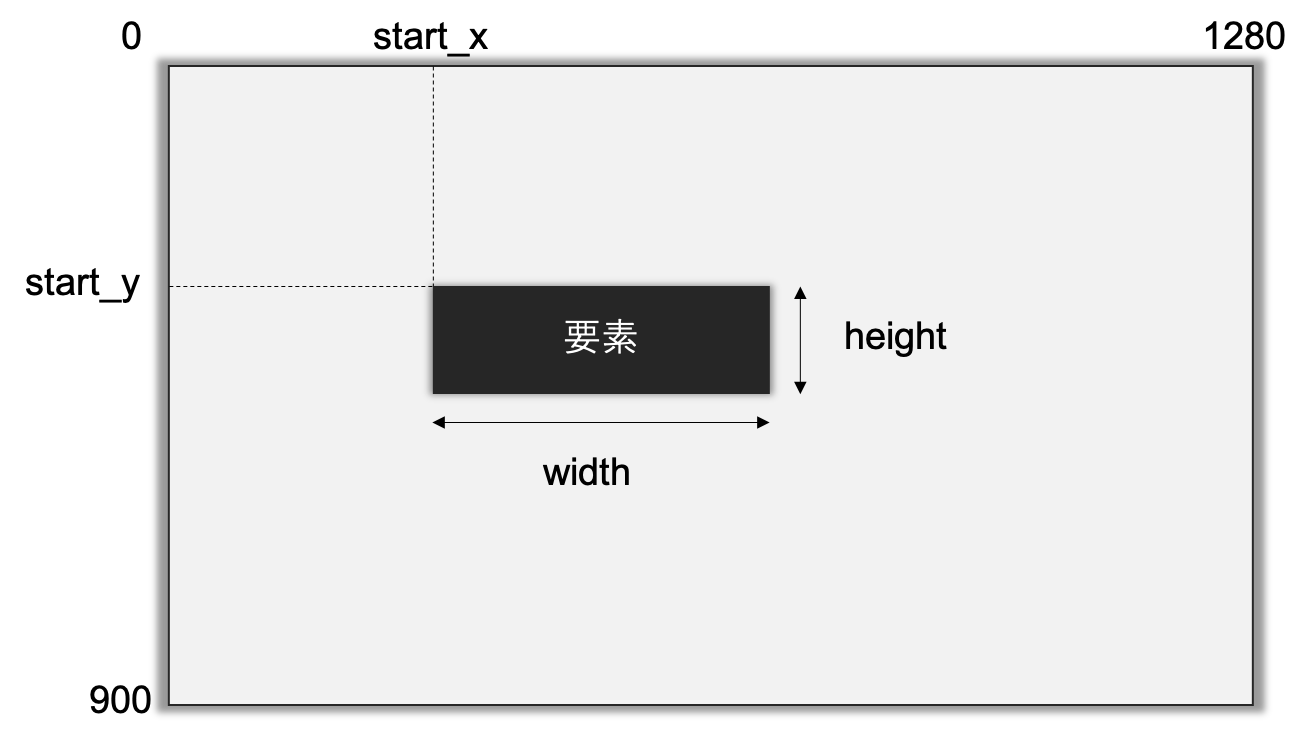
\includegraphics[width=8cm]{figures/getposition.png}
    \caption{基準点と要素の座標取得}
    \label{fig_getposition}
\end{figure}


\subsection{顕著度の計算}\label{subsec:system03}
% 領域のサイズ・位置による重み付けを行うことの記述・顕著度のランキングの取得方法
% F-bias Center-bias Webpage Saliencyより
% サイズによる重み付け
% 擬似プログラム
\par ここでは第\ref{subsec:system01}節で生成した顕著性マップと第\ref{subsec:system02}節で取得した各タグ要素の位置情報とサイズを比較して各要素の顕著度を計算する。顕著度の計算の流れを図\ref{fig_system03}に示す。

\begin{figure}[H]
    \centering
    
\includegraphics[width=12cm]{figures/system03.png}
    \caption{顕著度の計算の流れ}
    \label{fig_system03}
\end{figure}

\par まず始めに第\ref{subsec:system01}節で保存した顕著性マップを読み込む。使用端末により異なるが最近のパソコンは画面の高画質化が進み、横1280px縦900pxで撮影したスクリーンショットはその倍近い解像度で保存されている。その為、単純に顕著性マップを読み込み要素の位置情報と照らし合わせるとズレが生じてしまう。この問題を解決する為に読み込んだ顕著性マップを圧縮加工して取得した位置情報と同じサイズに合わせる必要がある。

\par 次に第\ref{subsec:system02}節で取得した各タグ要素毎に読み込んだ顕著性マップの該当要素の領域をトリミングする。また、トリミングした領域の色の明度の平均を計算する事で顕著度を計算する。しかしながら、単純に色の明度の平均を要素の顕著度にすると極端に小さな要素の顕著度が高く判定されてしまうなどの問題が生じた。そこで、本システムでは要素のサイズと位置による顕著度の重み付けを行う事でより正確に顕著度を判定出来るように工夫した。

\subsubsection{要素のサイズによる重み付け}\label{subsec:system03-1}
\par 先ほど述べた通り、単純に要素の明度の平均を取得すると小さな要素の顕著度が極端に高く計算される傾向があることが判明した為、要素の大きさによる重み付けを行うことで顕著度を平均化する。本来であれば深層学習等を用いて適切な重み付けを学習するのが良いが、本研究では実験を何度か行い極端に小さな要素の顕著度を低く判断する様に重み付けを独自の基準でアルゴリズム\ref{alg:weight-size}のように設定した。取得した要素の明度の平均値に重みをかける事で実装する。

\begin{algorithm}[H]
    \caption{サイズによる重み付け}
    \label{alg:weight-size}
    \begin{algorithmic}
    \Function{calc\_salient\_level}{start\_x, start\_y, size\_w, size\_h}
    \State salient\_level $ \leftarrow $ 要素の明度の平均値(0-255)
    \State salient\_level\_weight = size\_w * size\_h //要素の面積を計算
    \If{salient\_level\_weight $>$ 1000}
        \State salient\_level $ \leftarrow $ salient\_level
    \ElsIf{salient\_level\_weight $>$ 800}
        \State salient\_level $ \leftarrow $ salient\_level * 0.7
    \ElsIf{salient\_level\_weight $>$ 500}
        \State salient\_level $ \leftarrow $ salient\_level * 0.6
    \Else
        \State salient\_level $ \leftarrow $ salient\_level * 0.2
    \EndIf
    \State \Return salient\_level
    \EndFunction
    \end{algorithmic}
\end{algorithm}

\subsubsection{要素の位置による重み付け}\label{subsec:system03-1}
\par 関連研究でも触れたShenら\cite{shen2014webpage}の人間の目の視線を測定するアイトラッカーを用いてウェブページの顕著性を測定した実験によると、図\ref{fig_shen-experience}に示すようにテキスト中心と画像中心とテキスト画像が混合した全てのウェブページにおいて人は左上の領域と中心付近に目線が行く傾向が判明した。ウェブページの左上から中央にかけての領域に注目が集まるの現象はf-biasと言う名で一般的に知られており、本システムでも左上の領域と中心付近で顕著度が高くなるように重み付けを行う。

\begin{figure}[H]
    \centering
    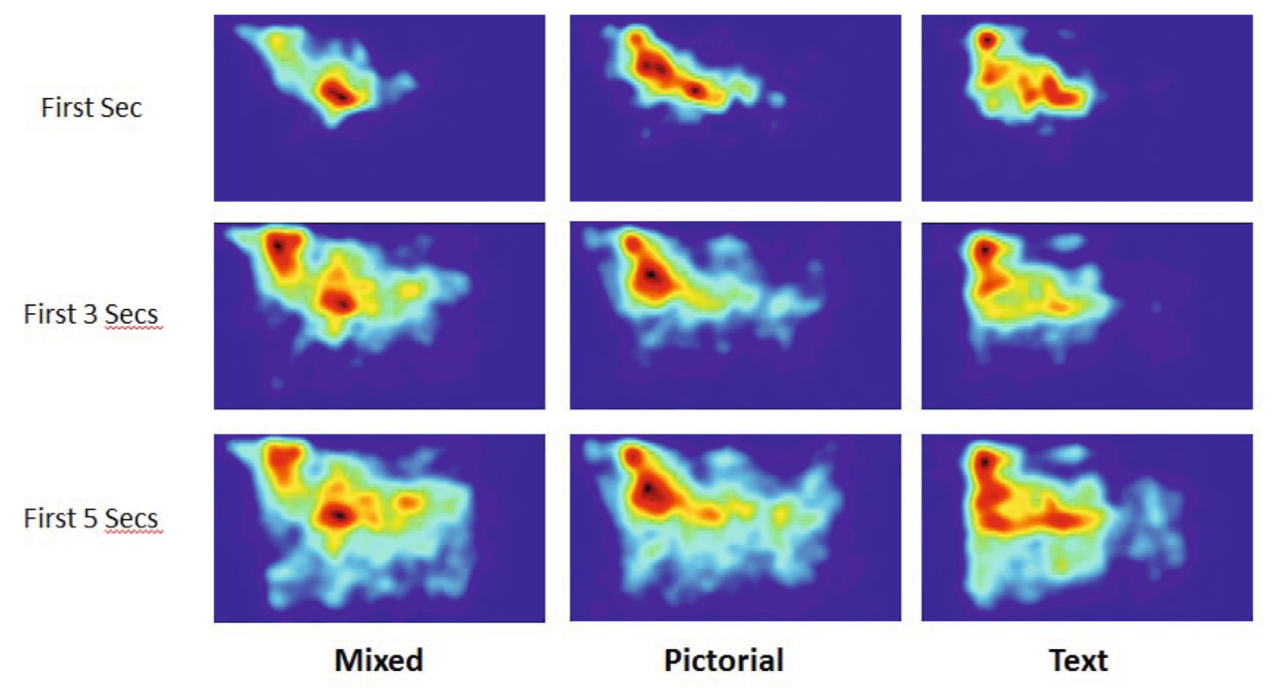
\includegraphics[width=8cm]{figures/shen-bias.png}
    \caption{Shenらのウェブページのヒートマップ生成実験結果\cite{shen2014webpage}}
    \label{fig_shen-experience}
\end{figure}

\par 本システムの位置情報による重み付けの手法をアルゴリズム\ref{alg:weight-position}に示す。要素の中心点の位置によって要素の顕著度の重み付けを行うことにした。左上の領域に大きな重みをつけるtop-left biasについては、横軸方向にどれだけの重みの差をつけるかを表すplace\_weight\_xと縦軸方向にどれだけの重みの差をつけるかを表すplace\_weight\_yの2つの数値を与える事で表現した。また、中心領域に大きな重みをつけるcenter biasにおいては中心部と最外部でどれだけ重みの差をつけるかを表すplace\_weight\_cを与える事で表現した。さらにtop-left biasとcenter biasを組み合わせる事で左上と中央部分に大きな重みをつけるf-biasを表現する。本研究においては横軸の重みの差を表すplace\_weight\_x = 0.1に縦軸の重みの差を表すplace\_weight\_y = 0.4に中心の重みの差を表すplace\_weight\_c = 0.2に設定した。正方形の20$\times$20マスのブロックをウェブページに見立てて重みの数値をシミュレーションした結果を図\ref{fig_fbias}に示す。左図はtop-left biasを、中央はcenter biasを、右図は2つを組み合わせたf-biasを表す。また、赤色に近くほど重みの数値が大きく白色に近くほど数値が小さいことを表す。さらに、図\ref{fig_fbias-test}にテスト用の同じ色の正方形を等間隔で並べたウェブページを入力した時の結果を示す。重み付け前の顕著性マップでは全ての正方形が同じ明度で表わされているが、重み付け後の顕著性マップでは左上から中央にかけての正方形の明度が高く表わされている事が確認できる。なお、認識しやすいように重み付け後の顕著性マップには顕著度のランキングを緑色の枠線の色で表している。

\par 最後に、要素毎に以上の重み付け処理を行なった結果の顕著度を最終的な出力に使用する為にCSVファイルに追記する。

\begin{algorithm}[H]
    \caption{位置情報による重み付け(F-bias)}
    \label{alg:weight-position}
    \begin{algorithmic}
    \Function{calc\_salient\_level}{start\_x, start\_y, size\_w, size\_h}
    \State salient\_level $ \leftarrow $ 要素の明度の平均値(0-255)
    \State width $ \leftarrow $ 顕著性マップの幅(px)
    \State height $ \leftarrow $ 顕著性マップの高さ(px) 
    \State place\_weight\_x $ \leftarrow $ 0.1 //横軸方向の重み
    \State place\_weight\_y $ \leftarrow $ 0.4 //縦軸方向の重み
    \State place\_weight\_c $ \leftarrow $ 0.2 //中心方向の重み
    \If{$size\_w < width$ and $size\_h < height$}
        \State x\_bias $ \leftarrow $ 1-(place\_weight\_x-((width-(start\_x+$\frac{size\_w}{2}$))*$\frac{place\_weight\_x}{width}$))
        \State y\_bias $ \leftarrow $ 1-(place\_weight\_y-((height-(start\_y+$\frac{size\_h}{2}$))*$\frac{place\_weight\_y}{height}$))
        \State top\_left\_bias $ \leftarrow $ x\_bias * y\_bias
        \State center\_bias\_x $ \leftarrow $ $|\frac{width}{2}-(start\_x+\frac{size\_w}{2})|^2$
        \State center\_bias\_y $ \leftarrow $ $|\frac{height}{2}-(start\_y+\frac{size\_h}{2})|^2$
        \State center\_bias $ \leftarrow $ $\sqrt{center\_bias\_x + center\_bias\_y} $
        \State salient\_level $ \leftarrow $ salient\_level*(topleft\_bias - (place\_weight\_c * center\_bias))
    \EndIf
    \State \Return salient\_level
    \EndFunction
    \end{algorithmic}
\end{algorithm}

\begin{figure}[H]
    \centering
    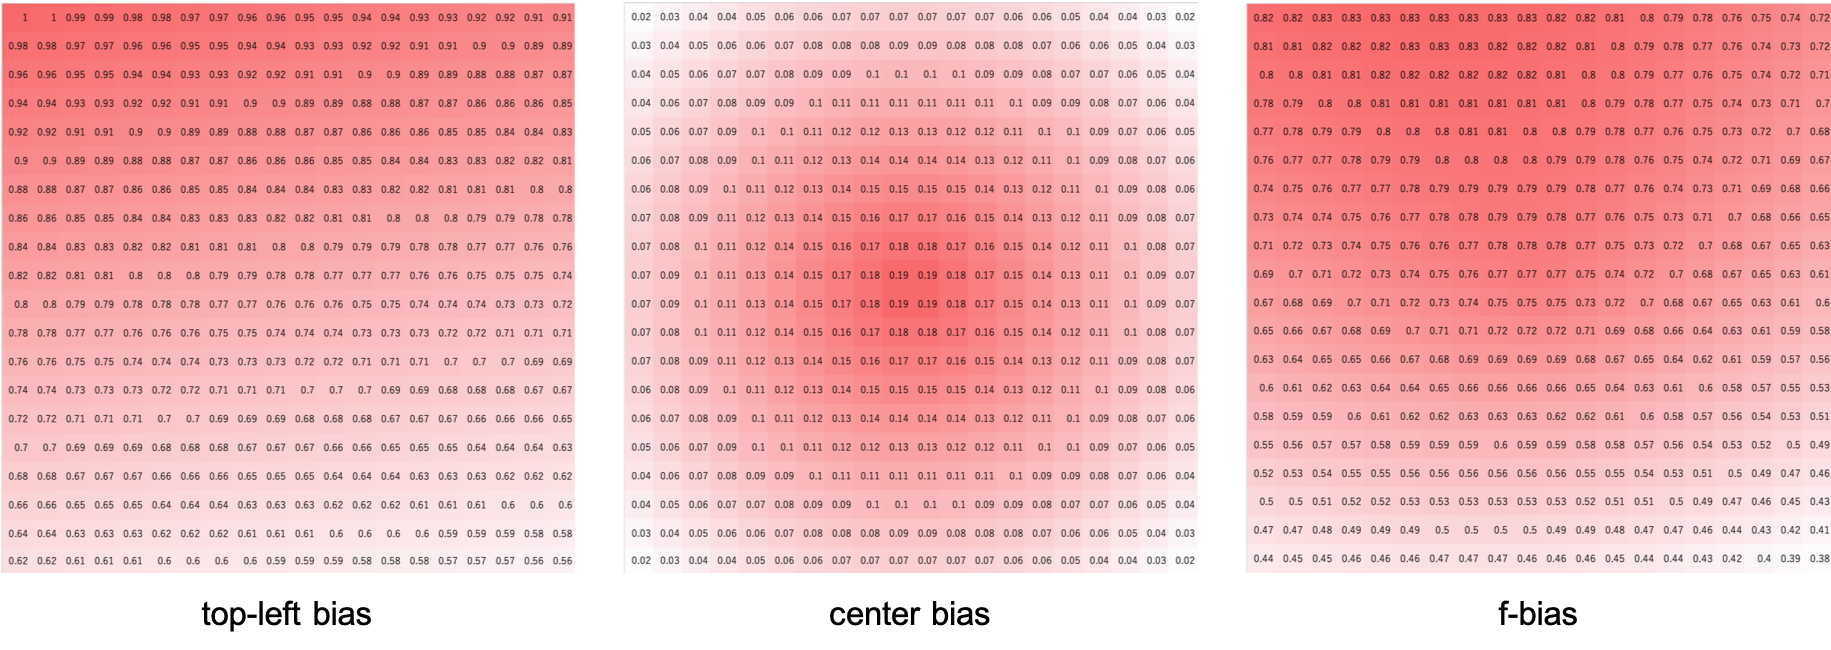
\includegraphics[width=12cm]{figures/fbias.png}
    \caption{位置情報による重み付けのシミュレーション}
    \label{fig_fbias}
\end{figure}

\begin{figure}[H]
    \centering
    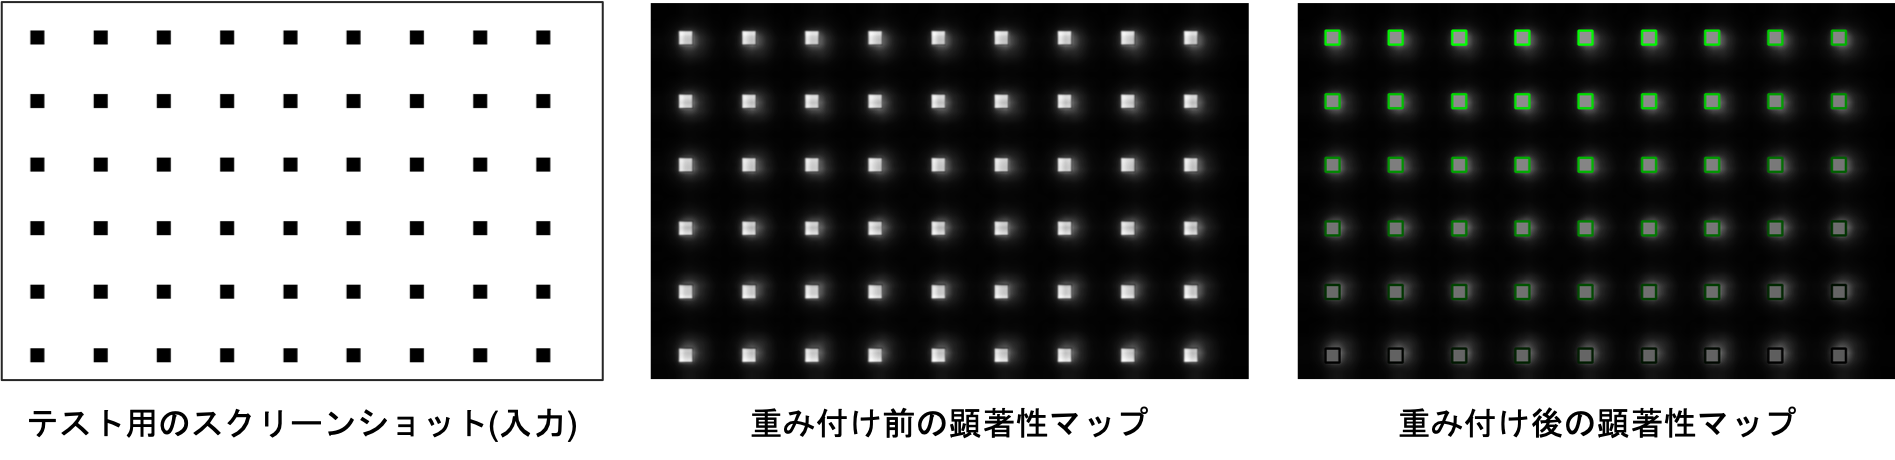
\includegraphics[width=12cm]{figures/fbias-test.png}
    \caption{テスト用ページを入力して得た顕著性マップ}
    \label{fig_fbias-test}
\end{figure}


\subsection{顕著領域の視覚化}\label{subsec:system04}
% 領域を塗りつぶして生成する顕著性マップと重要領域のランキングの生成方法の記述
\par ここでは第\ref{subsec:system03}節で計算した顕著度を元に顕著領域の視覚化を行う。本システムでは、顕著度が高い重要領域を要素単位で塗りつぶした顕著領域マップと特に顕著度が高い要素を一つにまとめた集約図の2つの出力を行う。顕著領域の視覚化の流れを図\ref{fig_system04}に示す。

\begin{figure}[H]
    \centering
    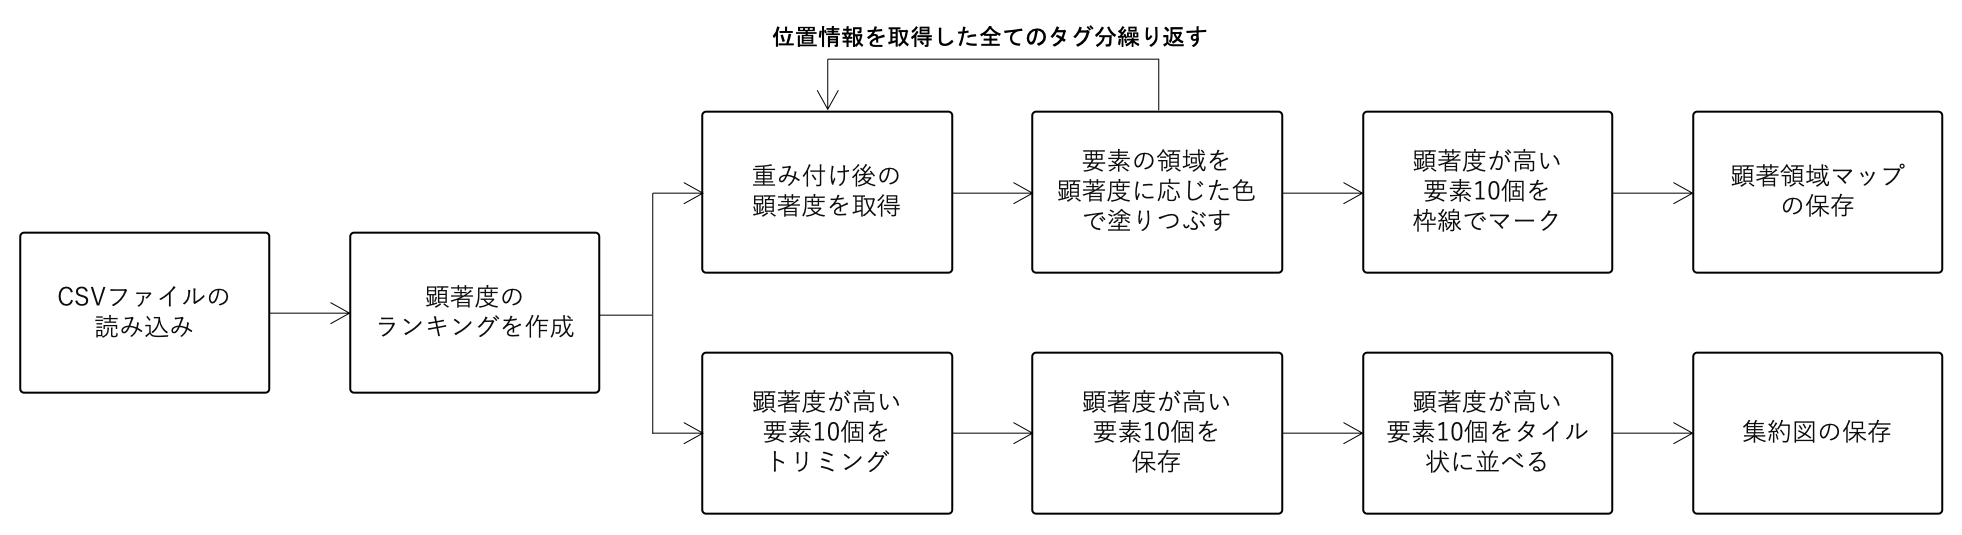
\includegraphics[width=12cm]{figures/system04.png}
    \caption{顕著領域の視覚化の流れ}
    \label{fig_system04}
\end{figure}

\subsubsection{顕著度ランキングの生成}\label{subsec:system04-1}
\par 顕著領域マップと集約図の生成にあたり、第\ref{subsec:system03}節で計算した顕著度のランキングを作成する。顕著度ランキングの計算アルゴリズムをアルゴリズム\ref{alg:lanking}に示す。まず始めに、第\ref{subsec:system03}節でCSVに保存した顕著度を顕著度が高い順にソートする。本来であれば、顕著度が高い順にランキングを付ければ良いが、図\ref{fig_system4-rank}に示すように同一要素を内包している他の要素も顕著度が高く評価されてしまう問題が生じる。同じ要素が顕著度ランキングに何度も出現する事は問題である為、一度顕著度が高いと評価した要素を内包する外部の要素をNGリストに格納して顕著度ランキングに入らないように評価する。



\newpage
\begin{algorithm}[H]
    \caption{顕著度ランキング}
    \label{alg:lanking}
    \begin{algorithmic}

    \State stag\_list $ \leftarrow $ CSVの読み組み, tag\_list\_num $ \leftarrow $ CSVの行数
    \State salient\_level = [] // 顕著度を格納するリスト, ng\_list = [] // NGリスト
    \State high\_element\_list = [] // 顕著度ランキングを格納するリスト
    \For{$i$ in $range(tag\_list\_num)$}
        \State salient\_level.append(tag\_listのi行目の要素の顕著度)
    \EndFor    
    \State salient\_level\_sort $ \leftarrow $ salient\_levelをソート
    \State salient\_num $ \leftarrow $ 10, temporal\_num $ \leftarrow $ 1, salient\_num\_first $ \leftarrow $ salient\_num

    \While{while salient\_num $>$ 0}
        \State most\_salient $ \leftarrow $ salient\_level\_sort[tag\_list\_num - temporal\_num]
        \If{(most\_salient in ng\_list) == False}
        \State start\_x, start\_y, end\_x, end\_y $\leftarrow$ CSVのmost\_salient行目から取得
        \State size $\leftarrow$ CSVからmost\_salient行目の要素のwidth $*$ heightを取得
        \If{(end\_x $-$ start\_x)/(end\_y $-$ start\_y) $<$ 10}
        \State high\_element\_list.append(most\_salient)
        \State salient\_num $\leftarrow$ salient\_num - 1
        \For{$i=1$ in $range(tag\_list\_num)$}
        \If{(most\_salient in ng\_list) == False}
        \State r\_start\_x, r\_start\_y, r\_end\_x, r\_end\_y $\leftarrow$ i行目から取得
        \State r\_size $\leftarrow$ CSVからi行目の要素のwidth*heightを取得
        \If{i行目要素とmost\_salient行目要素が内包関係}
        \If{r\_size $-$ size $<$ 200 $or$ size $-$ r\_size $<$ 200}
        \State ng\_list.append(i) //NGリストにi行目要素を格納
        \EndIf
        \EndIf
        \EndIf
        \EndFor 
        \EndIf
        \Else
        \State temporal\_num $\leftarrow$ temporal\_num $+$ 1
        \EndIf
    \EndWhile
    \end{algorithmic}
\end{algorithm}

\begin{figure}[H]
    \centering
    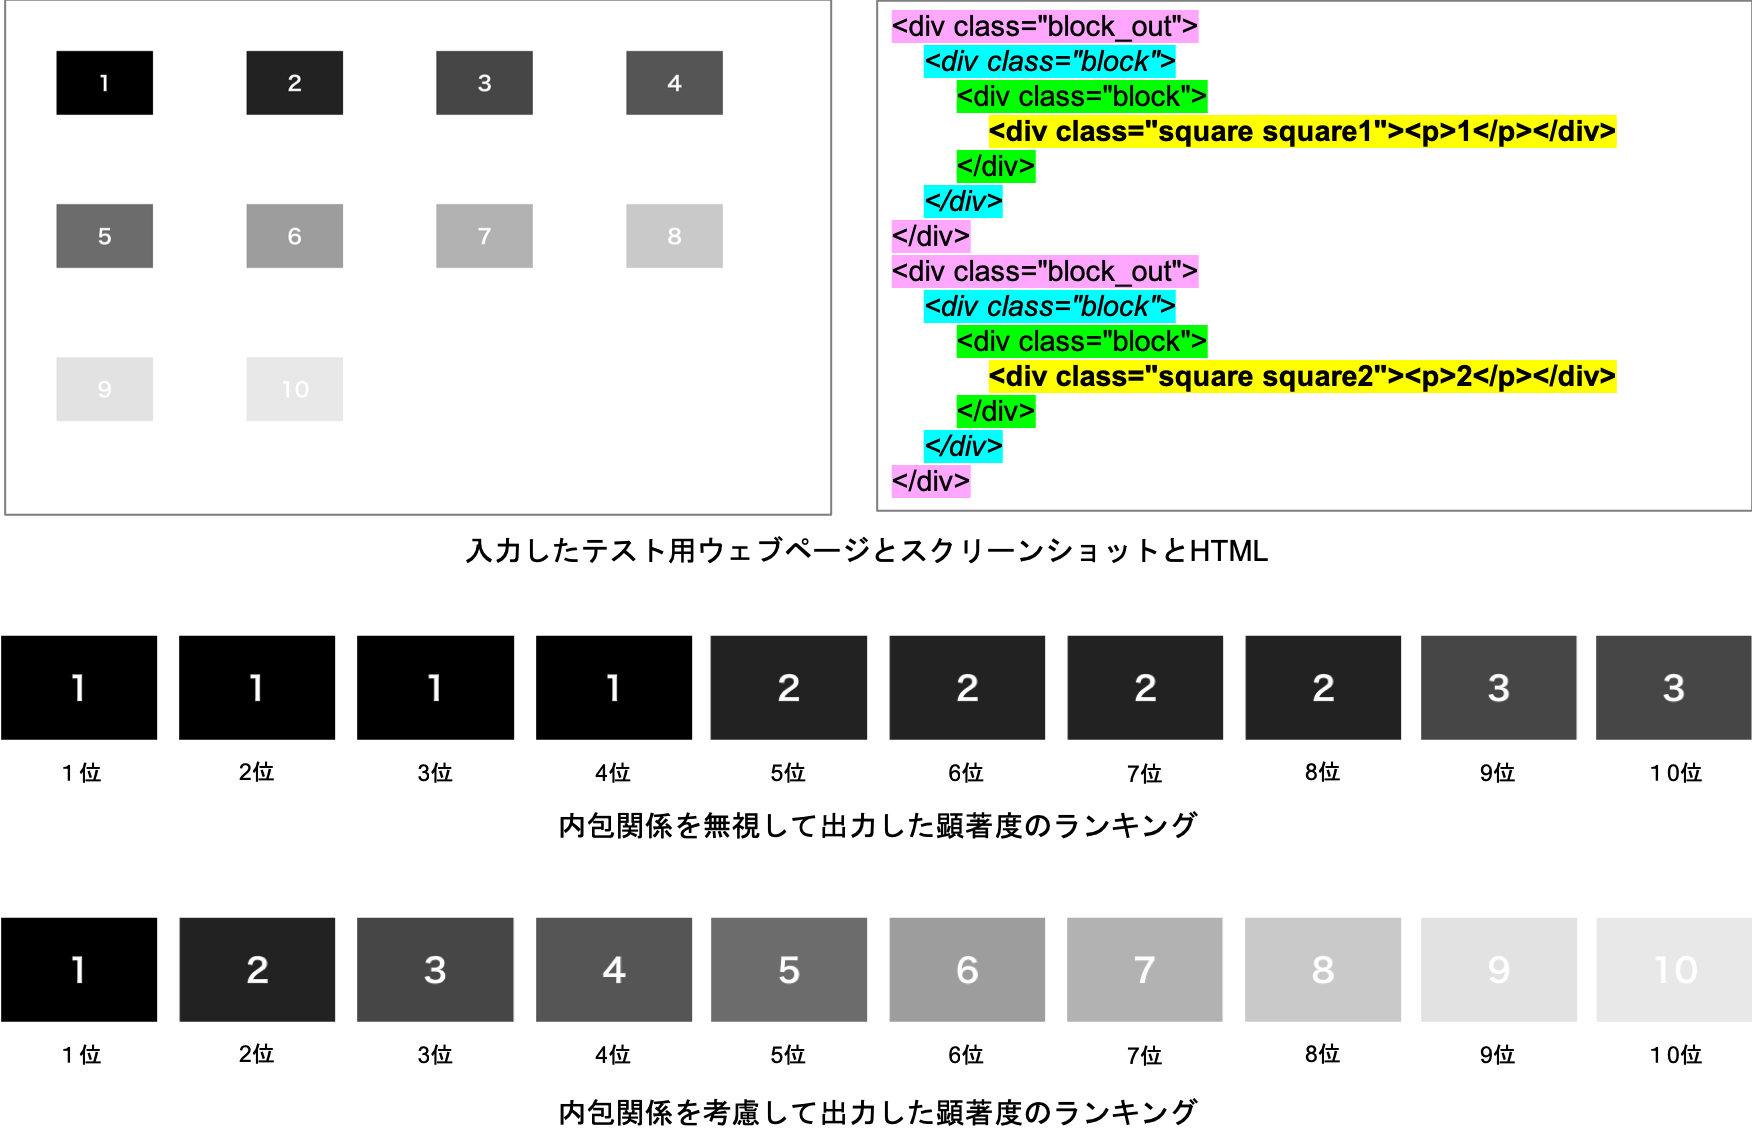
\includegraphics[width=12cm]{figures/include-rank.png}
    \caption{要素の内包関係を考慮した時としない時の顕著度ランキング}
    \label{fig_system4-rank}
\end{figure}

\subsubsection{顕著領域マップの生成}\label{subsec:system04-1}
\par 顕著領域マップの生成方法について説明する。第\ref{subsec:system03}節で計算した顕著度は0$\sim$255の範囲内の実数で表わされている。位置情報を取得した画面上に表示されている全ての要素の領域をこの顕著度を明度とした長方形で塗り潰す。また、第\ref{subsec:system03-1}節で説明した重み付けにより全体的に顕著度が低くなっている為、補正値を与える事ですべての要素の顕著度を補正値分高くすることとする。
\par さらに、特に顕著度が高い重要領域を視覚化する為に第\ref{subsec:system04-1}項で作成した顕著度ランキングの上位10個の要素の外枠を顕著度が高い順に明るい緑色の線で描写する。以上の作業を行う事で顕著領域マップの生成を行う。図\ref{fig_tile-example}に第\ref{subsec:system04-1}項で説明したテスト用ウェブページのURLを入力して生成された顕著領域マップの例を示す。

\subsubsection{集約図の生成}\label{subsec:system04-2}
\par 集約図の生成方法について説明する。第\ref{subsec:system04-1}項で作成した顕著度ランキングを元に顕著度が上位10個の要素の領域をスクリーンショットから切り取りタイル状に並べる。本システムでは上段に上位2個を、中段に3位$\sim$5位の3個を、下段には6位$\sim$10位の5個を並べる事で表現した。図\ref{fig_tile-example}に第\ref{subsec:system04-1}項で説明したテスト用ウェブページのURLを入力して生成された集約図の例を示す。


\begin{figure}[H]
    \centering
    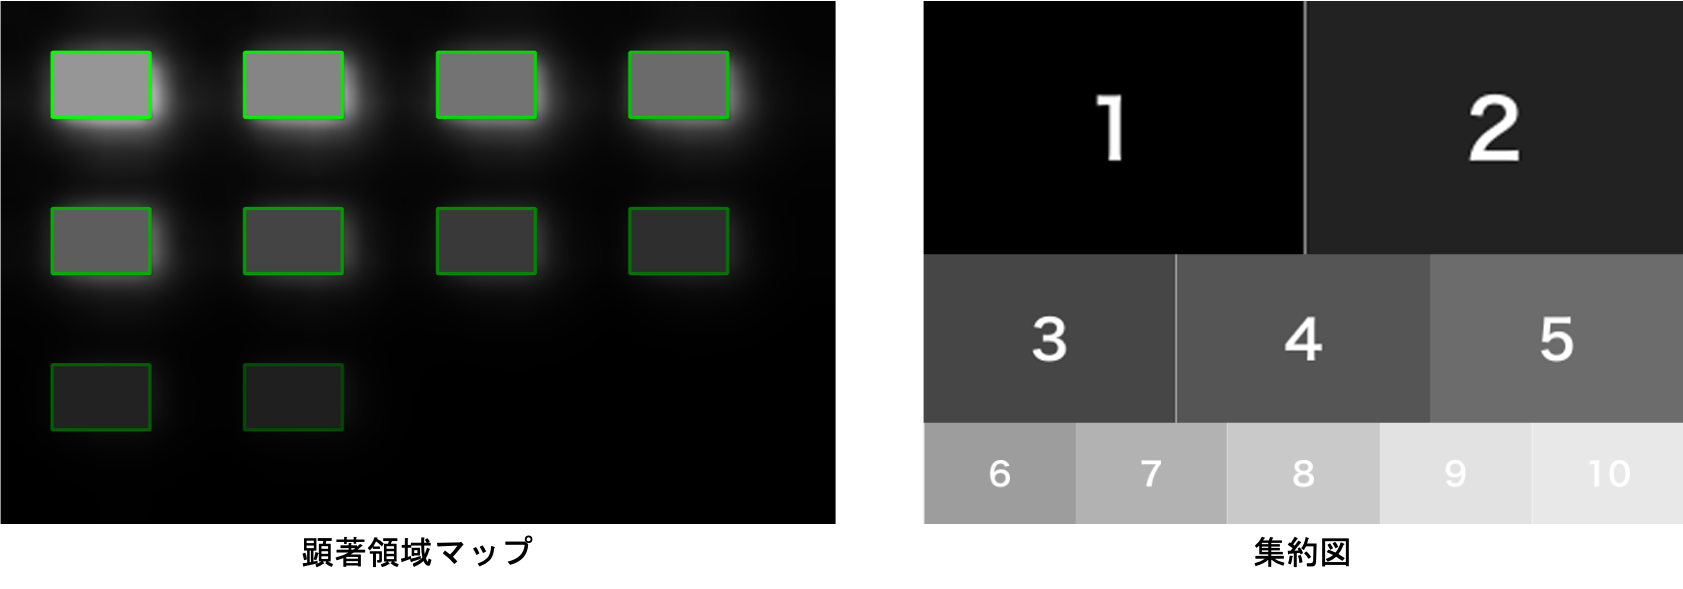
\includegraphics[width=10cm]{figures/example-output.png}
    \caption{生成される顕著領域マップと集約図の例}
    \label{fig_tile-example}
\end{figure}
% 第6章 本研究の詳細
\newpage
\renewcommand{\baselinestretch}{1.5}
\section{本研究の詳細}
\renewcommand{\baselinestretch}{1}

\par デザイナーやネットユーザーが検証するウェブページのURLおよびページのレイアウトタイプを入力すると該当ページの顕著性マップとページの構造を組み合わせることにより顕著度が高い領域を要素単位で分析して顕著領域マップを出力する手法を提案する。また、一般ユーザー向けに特に顕著度が高い領域を纏めて描写した集約図を出力する手法を提案する。本手法のモデルアーキテクチャを図\ref{fig_ourmodel}に示す。

\begin{figure}[H]
    \centering
    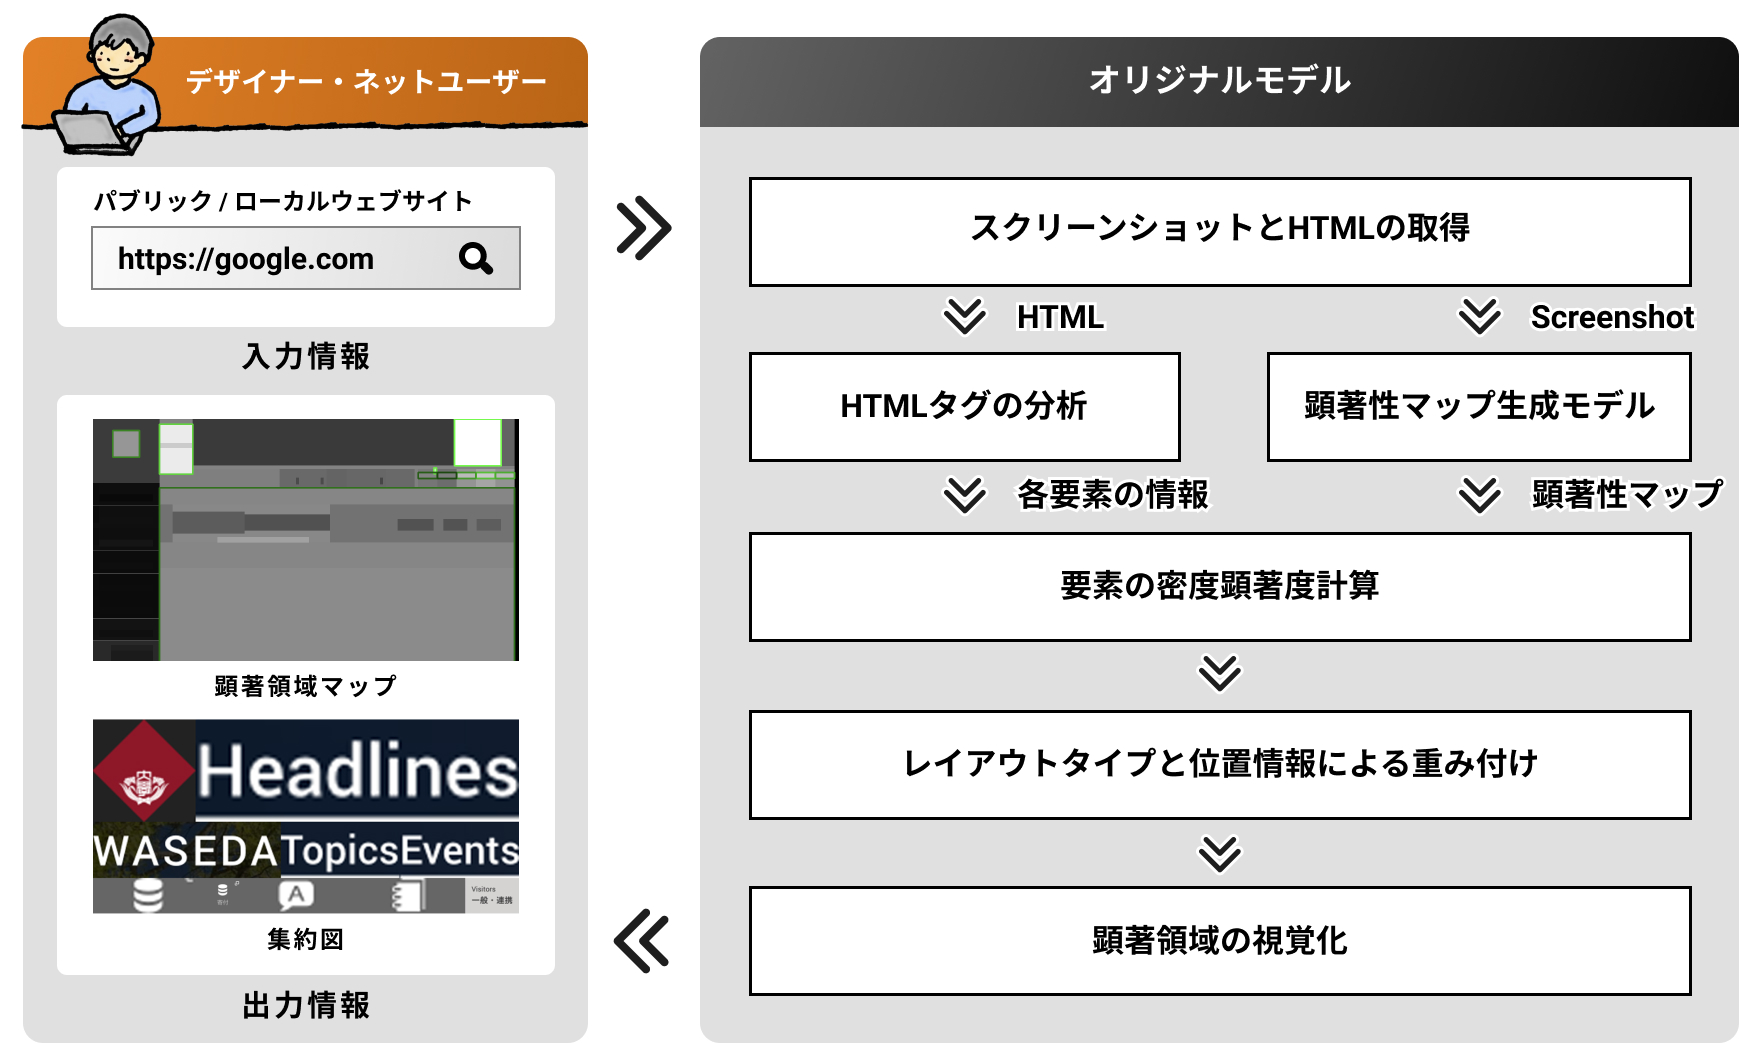
\includegraphics[width=9cm]{figures/model.jpg}
    \caption{モデルアーキテクチャ}
    \label{fig_ourmodel}
\end{figure}

\par 本手法の手順は大きく分けて以下の4つである。
\par(1) HTMLの取得と顕著性マップの生成
\par(2) HTMLの解析によるタグの分析と位置情報の取得
\par(3) レイアウトタイプを考慮した要素の顕著度計算
\par(4) 顕著領域の視覚化\\

\par なお、本研究ではサーバーサイドのプログラムを使用することで外部サーバーにアクセスしてウェブサイト上から必要な情報を取得するウェブスクレイピング技術としてウェブアプリケーションの自動テストツールであるSelenium WebDriver\cite{selenium}や取得したHTMLからタグや必要な情報を取得するPython用のライブラリであるBeautiful Soup\cite{beautifulsoup}を使用するが別のスクレイピング技術を使用しても実装は可能である。また、スクリーンショットを取得するウェブブラウザとしてFirefoxを使用するがChromeなど別のブラウザでも実装可能である。

\subsection{HTMLの取得と顕著性マップの生成}\label{subsec:system01}
\par 本システムではまず、入力されたURL情報を元にウェブスクレイピング技術を用いてスクリーンショットとHTMLを取得する。また、取得したスクリーンショットを用いて顕著性マップを生成する。デザイナーが開発段階で簡単に使用可能な様に入力するURLは、ネットワーク上に存在するウェブページだけでなくローカル環境のURLにも対応させている。HTMLの取得と顕著性マップの生成の流れを図\ref{fig_system01}に示す。

\begin{figure}[H]
    \centering
    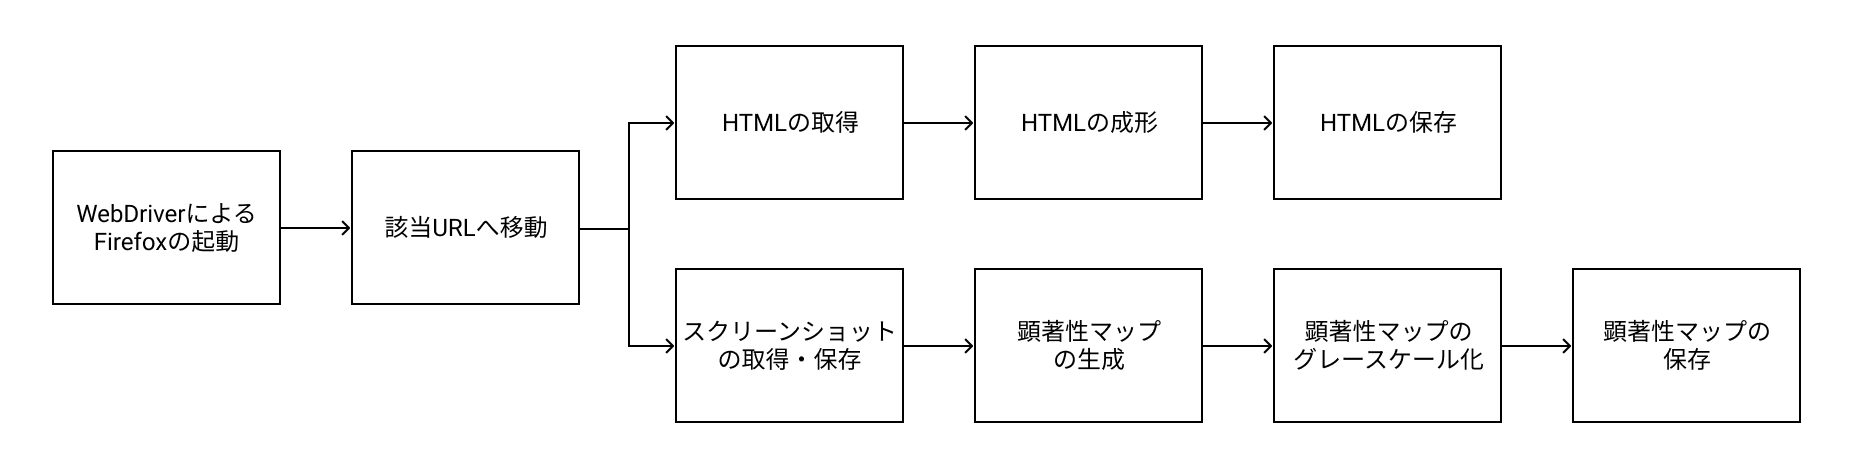
\includegraphics[width=12cm]{figures/06_process01.jpg}
    \caption{HTMLの取得と顕著性マップの生成の流れ}
    \label{fig_system01}
\end{figure}

\par まず始めに、Selenium WebDriverを用いてFirefoxを起動し、ブラウザのウィンドウサイズを一般的なパソコンで閲覧する条件に近い横1280px縦900pxに設定する。次に入力されたURLにアクセスを行い、ウェブページの読み込みが完了したらHTMLの取得を行う。取得したHTMLはインデントなどが乱れた状態である為、Selenium WebDriverと同じくウェブスクレイピング技術のライブラリであるBeautiful Soup\cite{beautifulsoup}を使用して扱いやすい状態に整形を行った後に保存する。

\par 次にウェブページのスクリーンショットを取得する。取得するスクリーンショットは、重要度が高いコンテンツはウェブページの最上部に存在する可能性が高いという考えから、ウェブページにアクセスした時点で閲覧可能な最上部の横1280px縦900pxとした。さらに、取得したスクリーンショットから顕著性マップを生成する。顕著性マップの生成には人間の目の視覚認識と同様に色・輝度・方向のそれぞれの視覚特徴を抽出した後に重み付けして足し合わせることにより顕著性マップを生成する最もベーシックなモデルのItti-Kochらの顕著性マップ生成モデルをベースに使用した。顕著性マップ生成モデルには深層学習を使用した精度の高いモデルまで幅広く存在しているが、特にバイアスを考慮しておらず扱いやすいモデルを使用することにした。
\par ここで顕著性マップ生成モデルにより出力される顕著性マップはRGBの3色チャンネルで出力されるが、計算処理を行いやすいように単色チャンネルで表されるグレースケール画像に変換して保存する。図\ref{fig_06_example_saliencymap}に早稲田大学ウェブサイトトップページ(2021年1月時点)\cite{waseda_top}のスクリーンショットを入力した時に生成される取得されるグレースケール顕著性マップの例を示す。

\begin{figure}[H]
  \centering
  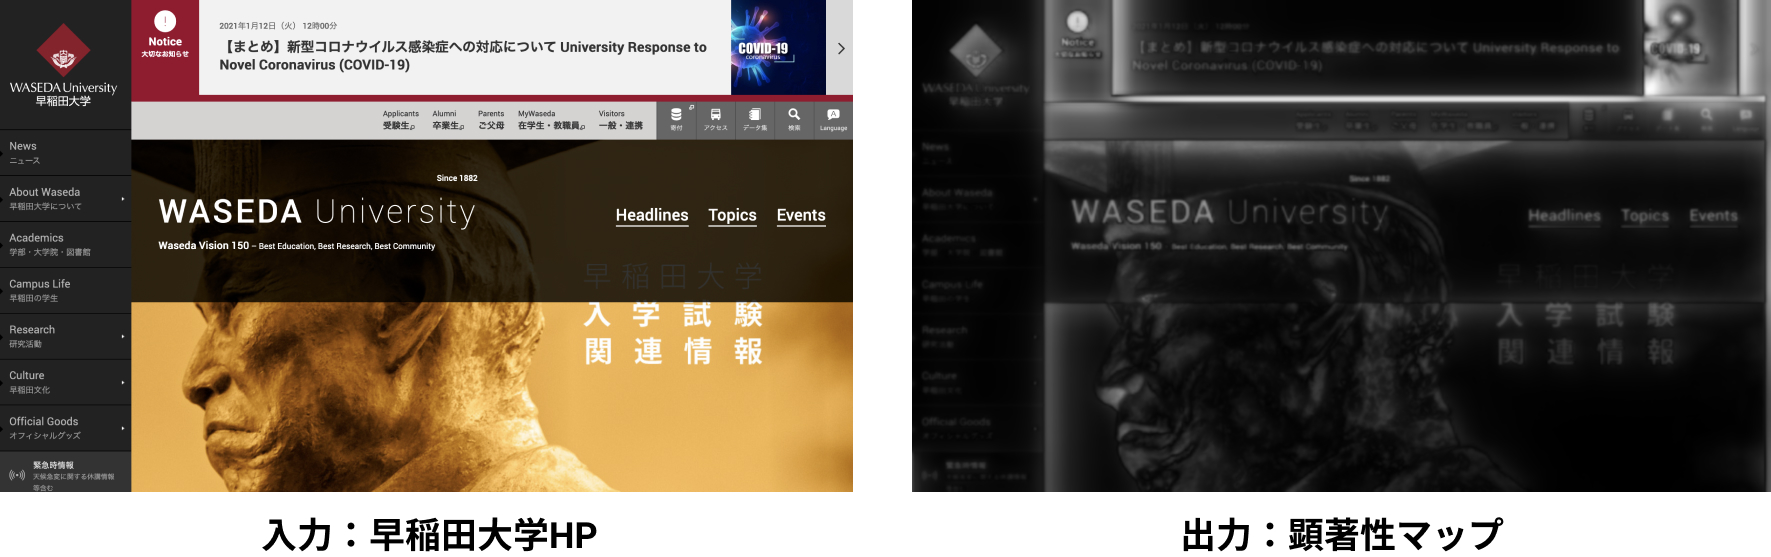
\includegraphics[width=12cm]{figures/06_ex-saliencymap}
  \caption{出力されるウェブページの顕著性マップの例}
  \label{fig_06_example_saliencymap}
\end{figure}


\subsection{HTMLの解析によるタグの分析と位置情報の取得}\label{subsec:system02}
\par ここでは第\ref{subsec:system01}節で取得したHTMLの解析を行いウェブページ上の要素の位置情報とそのサイズを取得する。HTMLの解析によるタグの分析と位置の取得の流れを図\ref{fig_system02}に示す。

\begin{figure}[H]
    \centering
    
\includegraphics[width=12cm]{figures/06_process02.jpg}
    \caption{HTMLの解析によるタグの分析と位置の取得の流れ}
    \label{fig_system02}
\end{figure}

\par まず始めに第\ref{subsec:system01}節で取得したHTMLの分析を行い、Selenium WebDriverで表\ref{table:gettaglist}に示す7個のタグ要素のidまたはclass名と左上の頂点の座標と縦と横のサイズを取得してそれらの情報をデータベースに記録する。各要素の座標の取得方法については、ウェブブラウザの表示領域の左上を基準点(0,0)として基準点からの距離を要素の座標とした。また、時間短縮とエラーを防ぐために取得したスクリーンショット領域内に表示されている要素のみを取得する。早稲田大学ウェブサイトトップページ(2021年1月時点)\cite{waseda_top}および、Yahoo! JAPANトップページ(2021年1月時点)\cite{yahoo}のウェブページの要素情報を取得して、直線で各要素を囲んだ例を図\ref{fig_06_ex-lineview}に示す。表示領域の指定要素のサイズと位置を取得している事が確認できる。

\begin{table}[h]
    \caption{位置情報とサイズを取得するタグの一覧}
    \label{table:gettaglist}
    \centering
     \begin{tabular}{clll}
      \hline
      要素名 & タグ & 意味 \\
      \hline \hline
      ブロック要素 & \textless div\textgreater & ブロック要素を表す \\
      見出し1 & \textless h1\textgreater & 文書中の見出しを示す為の要素で最も重要 \\
      見出し2 & \textless h2\textgreater & 文書中の見出しを示す為の要素で2番目に重要 \\
      見出し3 & \textless h3\textgreater & 文書中の見出しを示す為の要素で3番目に重要 \\
      リンク & \textless a\textgreater & リンクを示す \\
      インライン要素 & \textless span\textgreater & インライン要素を示し、重要な要素が多い \\
      段落 & \textless p\textgreater & テキスト要素を表す \\
      入力欄 & \textless input\textgreater & フォームなどの入力要素を表す \\
      イメージ & \textless img\textgreater & 画像要素を表す \\
      \hline
    \end{tabular}
\end{table}

\begin{figure}[H]
  \centering
  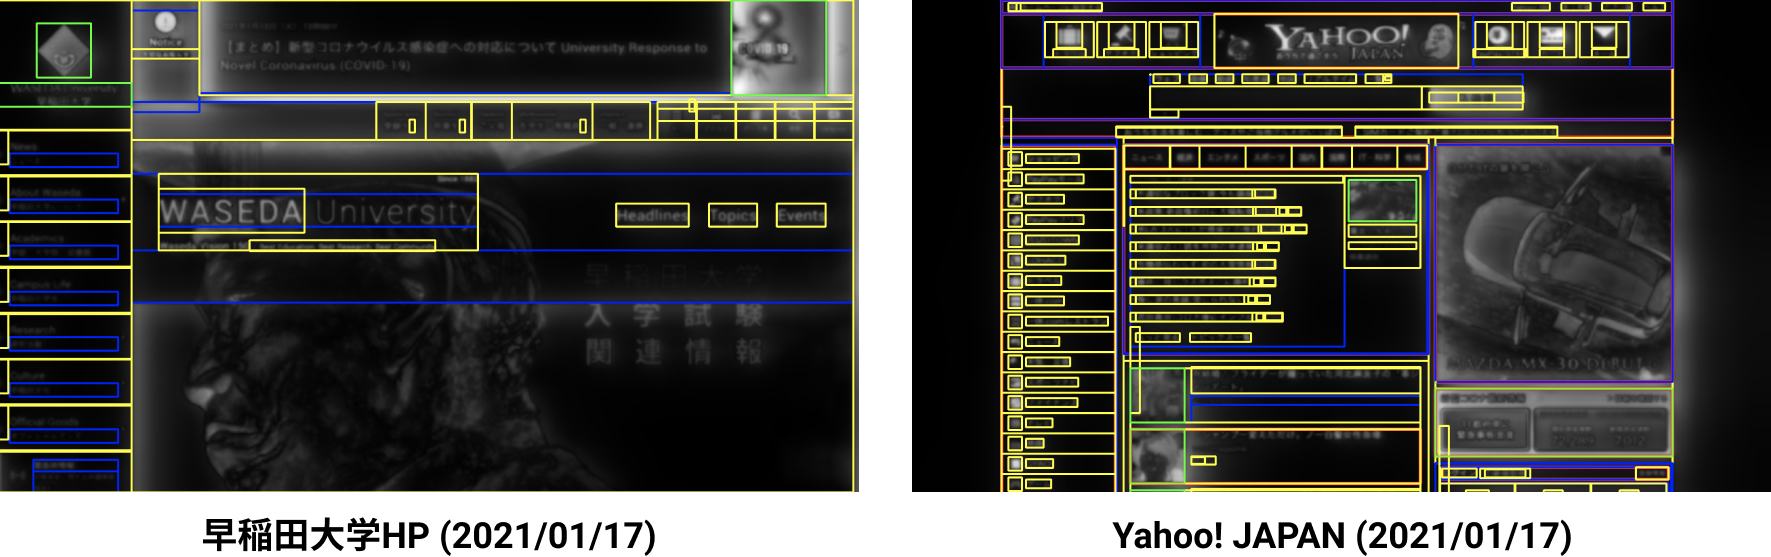
\includegraphics[width=12cm]{figures/06_ex-lineview.jpg}
  \caption{ウェブページの要素の取得の様子}
  \label{fig_06_ex-lineview}
\end{figure}

\subsection{レイアウトタイプを考慮した要素の顕著度計算}\label{subsec:system03}
\par ここでは第\ref{subsec:system01}節で生成した顕著性マップと第\ref{subsec:system02}節で取得した各要素の位置情報とサイズを組み合わせて各要素の顕著度を計算する。レイアウトタイプを考慮した要素内顕著度の計算の流れを図\ref{fig_system03}に示す。

\begin{figure}[H]
    \centering
    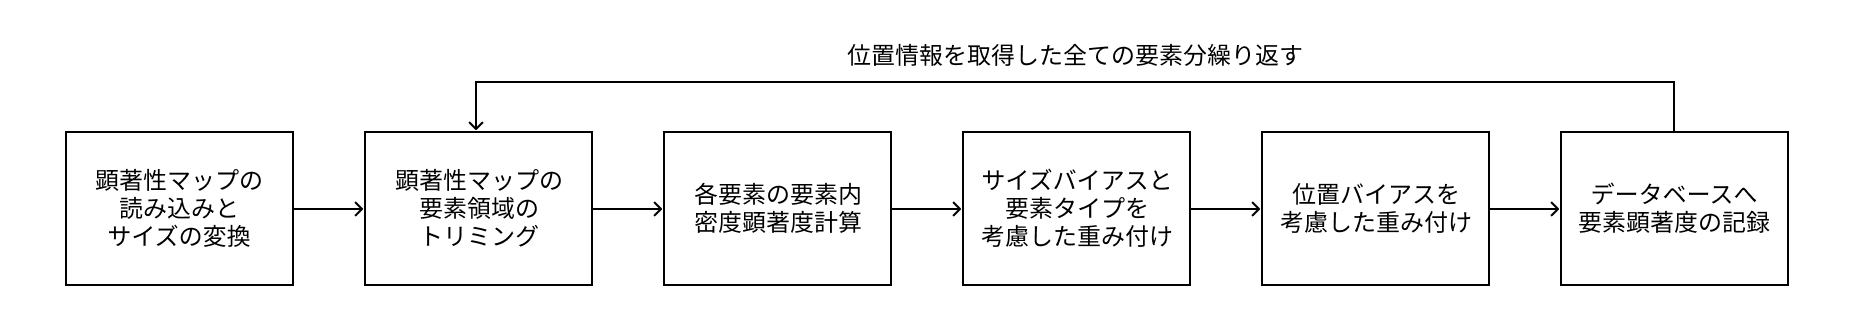
\includegraphics[width=12cm]{figures/06_process03.jpg}
    \caption{顕著度の計算の流れ}
    \label{fig_system03}
\end{figure}

\par まず始めに第\ref{subsec:system01}節で作成した顕著性マップを読み込む。使用端末により異なるが最近のパソコンは画面の高画質化が進み、AppleのRetinaディスプレイなどの高精細ディスプレイでは複数のピクセルで1つのドットを表しており倍近い解像度でスクリーンショットが保存されている。その為、単純に顕著性マップを読み込み要素の位置情報と照らし合わせるとズレが生じる。この問題を解決する為に読み込んだ顕著性マップを圧縮して実際にウェブブラウザ上で取得した位置情報と同じサイズに合わせる必要がある。

\par 次に第\ref{subsec:system02}節で取得した各要素ごとの顕著度を計算するために顕著性マップの該当要素の領域をトリミングする。また、トリミングした領域のピクセルレベルでの顕著度の積分を要素面積の平均顕著度で割る事で要素の密度顕著度を計算する。具体的な計算方法をアルゴリズム\ref{alg:element_saliency}に示す。従来は要素内部のピクセルレベルの顕著度の平均を顕著度としていたが、要素のピクセルレベルでの密度顕著度を計算したことで、小さな要素から大きい要素までバランスよく顕著度を評価する事が可能である。

\par しかしながらアイコンなどの極端に小さい要素の顕著度が過剰に高く評価されてしまうなどの問題が生じた。またウェブページの左上から中央にかけての領域に視線が集まりやすいf-biasなどのウェブページ固有の現象なども存在する。それらの問題を解決するために、本システムでは要素のサイズと位置情報によるレイアウトを考慮した顕著度の重み付けを行う事でより正確に顕著度を判定出来るように工夫した。

\begin{algorithm}[H]
  \small
  \caption{要素の顕著度計算手法}
  \label{alg:element_saliency}
  \begin{algorithmic}
  \Function{get\_element\_salient\_level}{start\_x, start\_y, end\_x, end\_y}
  \If{(end\_x - start\_x) $>$ 0 and (end\_y - start\_y) $>$ 0}
    \State cliped = Element.canvas.cv2[start\_y:end\_y, start\_x:end\_x] //要素をトリミング
    \State element\_occupancy = $\frac{(end\_x - start\_x) \times (end\_y - start\_y)}{width * height}$ //要素の占有率を計算
    \State salient\_level = $\frac{get\_element\_total\_saliency(cliped)}{get\_total\_saliency() \times element\_occupancy}$ //要素の顕著度を計算
    \State \Return salient\_level
  \Else
    \State \Return 0
  \EndIf
  \EndFunction
  \State
  \Function{get\_total\_saliency}{}
    \State clipped = Element.canvas.cv2[0:height, 0:width] //ウェブページ全体
    \State total\_saliency\_per\_row = np.sum(clipped, axis=0) //行の色の合計を取得
    \State total\_saliency = np.sum(total\_saliency\_per\_row, axis=0) //列の色の合計を取得
    \State \Return np.uint8(total\_saliency)
  \EndFunction
  \State
  \Function{get\_element\_total\_saliency}{clipped}
    \State total\_saliency\_per\_row = np.sum(clipped, axis=0) //行の色の合計を取得
    \State total\_saliency = np.sum(total\_saliency\_per\_row, axis=0) //列の色の合計を取得
    \State \Return np.uint8(total\_saliency)
  \EndFunction
  \end{algorithmic}
\end{algorithm}

\subsubsection{要素のサイズと要素タイプによる重み付け}\label{subsec:system03-1}
\par 先ほど述べた通り、アイコンなどの極端に小さい要素の顕著度が極端に高く計算される傾向があることが判明した為、要素の大きさによる重み付けを行うことで顕著度の偏りをなくす。ウェブページに存在するアイコンには様々なサイズのものが存在する。また画像要素だけでなく、CSSで描写されたアイコンやdiv要素にbackgroundプロパティで指定されたものなど要素のタイプも様々である。そこで本システムでは一般的にアイコンと呼ばれるサイズ以下の要素の重みを変更して適切な顕著度を計算する事にした。

\par 我々が日常でよく閲覧するアイコンとしてWindowsやMacやIOSなどのOS標準のアイコンが存在する。MicrosoftによるとWindowsではダイアログボックスやエラーページなどに32px$\times$32pxのアイコンが標準サイズとして使用されている\cite{windowsicon}。また、iPhoneなどのIOSやMacには64px$\times$64pxのアイコンが標準サイズとして使用されている\cite{appleicon}。日常でよく使用するアイコンのサイズのほとんどは32px$\times$32pxおよび64px$\times$64pxであることから人はこれらのサイズの要素をアイコンと認識する傾向が高い。以上のことから本システムでは64px$\times$64px以下のサイズの要素をアイコン要素とみなして顕著度を低く重み付けするようにアルゴリズムを\ref{alg:weight-size}のように設定した。なお、重み付けの値については本来であれば深層学習等を用いて適切な重み付けを学習するのが良いが、極端に小さな要素の顕著度を適切に判断できるように様々な値で繰り返し実験を行い最も実際の顕著度に近くなった値を設定した。

\begin{algorithm}[H]
  \small
  \caption{サイズによる重み付け}
  \label{alg:weight-size}
  \begin{algorithmic}
  \Function{apply\_size\_bias}{salient\_level, start\_x, start\_y, end\_x, end\_y}
  \State element\_area =  (end\_x - start\_x) $\times$ (end\_y - start\_y) //要素の面積を計算
  \If{element\_area $>$ 64 $\times$ 64 }
    \State salient\_level = salient\_level
  \Else
    \State salient\_level = salient\_level $\times$ 0.5
  \EndIf
  \State \Return salient\_level
  \EndFunction
  \end{algorithmic}
\end{algorithm}

\begin{figure}[H]
  \centering
  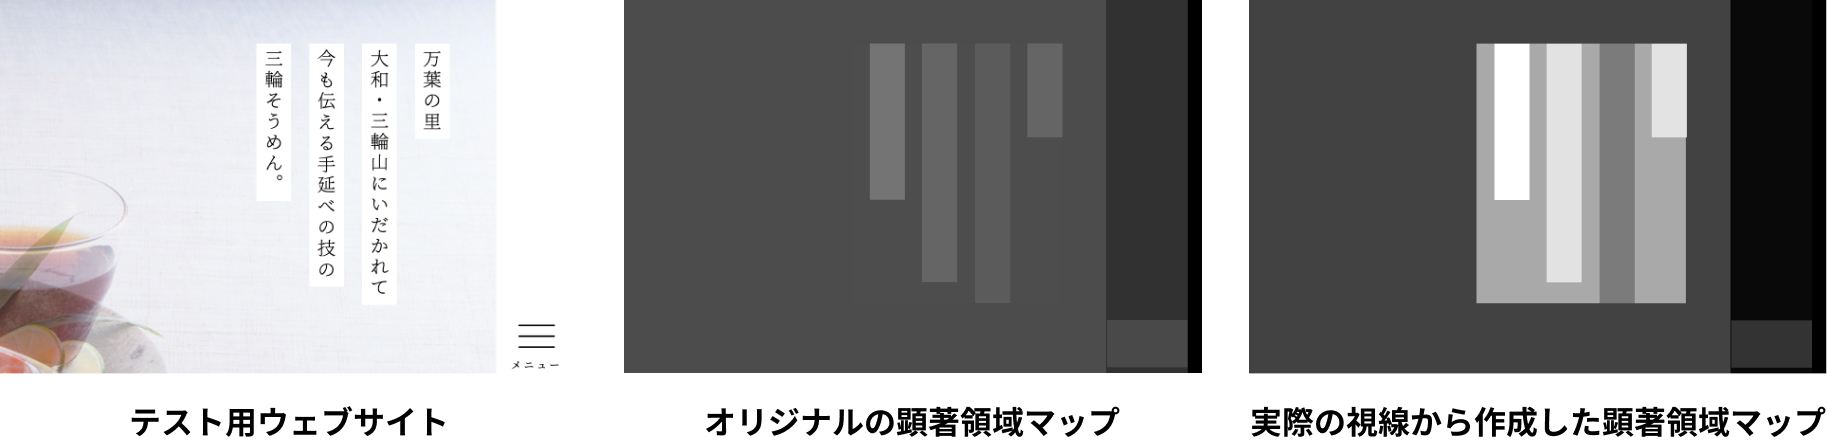
\includegraphics[width=12cm]{figures/06_textbias.jpg}
  \caption{テキスト箇所の顕著性評価比較}
  \label{fig_textbias}
\end{figure}

\par ウェブページには自然画像とは異なり様々なウェブページ固有の要素が存在する。その中の一つであるテキスト要素は自然画像にはほとんど存在せずあまり顕著度が高く評価されないがウェブページには多く存在する。図\ref{fig_textbias}にウェブページのテキスト表示箇所のオリジナルモデルの顕著領域マップと実際の視線データから作成した顕著領域マップの比較を示す。図から分かる通り人はテキスト要素に注目する傾向が高いが、Itti-Kochらのモデルなどの自然画像向け顕著性マップ生成モデルはテキストの顕著度をあまり高く評価しない。テキスト要素の顕著度を正しく評価するために該当要素の顕著度を高くするように重み付けを行った。


\subsubsection{要素の位置とレイアウトによる重み付け}\label{subsec:system03-2}
\par 関連研究でも触れたが有名なものとしてウェブページには自然画像と異なり、左上から中央付近の領域に存在する要素が注目されやすい傾向があるf-biasというバイアスが存在する。図\ref{fig_gazetime}に第\ref{subsec:gazedataset}節で作成した被験者がデータ分析用のウェブページを10秒間閲覧した際の実際の視線座標データを3秒間ずつヒートマップに表したものを示す。一番右の10秒間全ての視線座標データを合成したヒートマップを見ると左上から中央付近の要素に注目が集まりやすい傾向があるのは明らかである。また時間帯ごとの視線座標の推移を確認すると、最初の3秒間は左上から中央の領域が顕著に注目されている事が確認できる。また、3000ms-6000msや6000-9000msのヒートマップを見ると時間が経過するにつれて被験者の視線は左上から中央付近にかけて移動してより幅広い範囲に広がっている事が確認できる。このように昔からのベーシックデザインだけでなく近年の主流になっているモダンデザインにおいてもf-biasが適応可能である。また、時間の経過につれて注目される領域が大きく変化する事が明らかになった。

\begin{figure}[H]
  \centering
  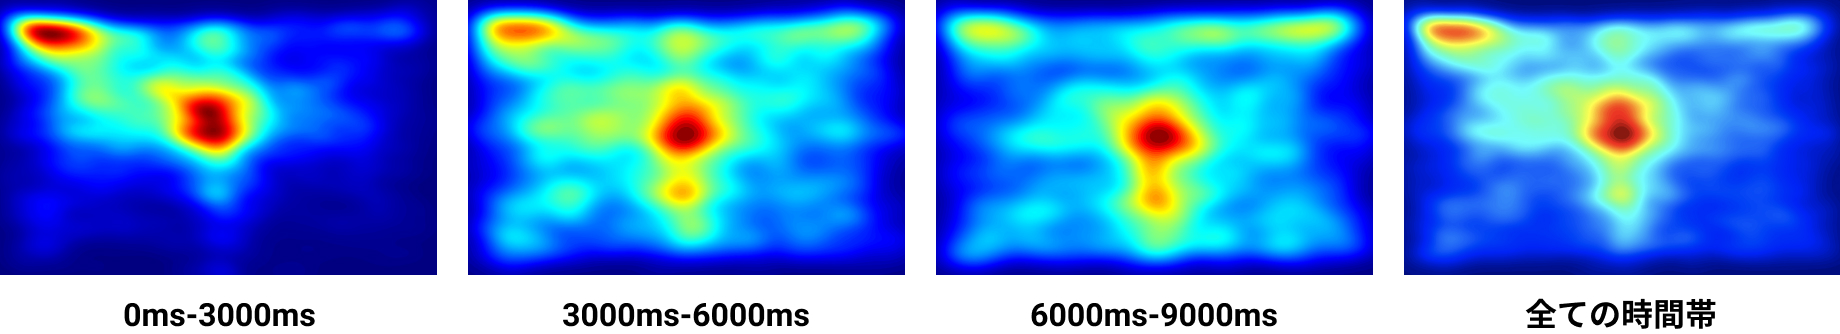
\includegraphics[width=12cm]{figures/06_gazetime.jpg}
  \caption{各時間帯ごとの平均顕著性ヒートマップ}
  \label{fig_gazetime}
\end{figure}

\par このようなウェブページ固有の視線のバイアスを反映させる為に本システムでは要素の位置情報ならびにウェブページのレイアウトタイプによる重み付けを行う。従来の研究では左上の領域に大きな重みをつけるtop-left biasを横軸方向と縦軸方向にそれぞれ重みを付ける事で擬似的に表現していた。また、中心領域に大きな重みをつけるcenter biasにおいては中心部と最外部でどれだけ重みの差をつけるかを表す重みを設定する事で表現していた。しかしながらこれらの手法では全てのレイアウトにおいて同じ擬似的なバイアスを適応させることになり顕著度評価の正確性はあまり高くない。そこで本研究ではレイアウトタイプによる重み付けを行い、各レイアウトごとの視線データの推移の傾向を分析して結果を適応する。図\ref{fig_layout_result}に各レイアウトに所属するウェブページの中央点とその移動の軌跡を示す。図\ref{fig_layout_result}の×マークはそれぞれのレイアウトに所属する各ウェブページの2秒間の視線座標の平均座標である。また大きく外れているものを除いて各ウェブページの平均座標の全てが含まれるように作成された楕円の中心座標を中央点と呼び、ウェブページ上の要素の中心がこの楕円の中に含まれる場合は閲覧される可能性が高いことを示す。なお、10秒間の閲覧を2秒ごとに区切ることで各時間帯ごとの視線の推移を確認する事が可能である。シングルカラムパターンや2カラムパターンなどのカラムレイアウトは左上の領域から中央の領域にかけて注目されている一方で、ブロークングリッドパターンやフルスクリーンパターンなどのモダンデザインレイアウトは時間の経過による視線の動きはあまり大きくなく、中央付近の要素が注目されやすい。これらの特徴を利用して位置情報とレイアウトによる重み付けを行う。本システムの重み付けの手法をアルゴリズム\ref{alg:weight-position}に示す。

\par まず初めに調査対象のウェブページのレイアウトの顕著領域情報を表\ref{table:layoutresult}より取得する。次にウェブページの各要素の中心座標が取得した顕著領域の中に入っているかどうかを$judge\_inside\_ellipse$関数で調査する。調査方法については、2秒ごとの合計5つの時間帯の楕円顕著領域のいずれかに要素の中心座標が存在するかどうかを確認して存在する場合は注目される可能性が高いことを示す。注目される可能性が高い要素については反復実験から決定した位置バイアスの重み$weight\_position$を乗算することで要素の顕著度の重み付けを行う。

\par 図\ref{fig_positionbias}にテスト用ウェブページを入力した時の各レイアウトの要素の位置情報による重み付けのシミュレーション結果を示す。テスト用ウェブページは左上の画像のように白色の背景上に黒色の正方形を等間隔で並べたものを使用した。最上部中央の画像のように重み付け前の顕著性マップでは全ての正方形が同じ明度で表わされているが、位置情報による重み付け後の顕著性マップでは第\ref{subsec:gazedataset}節で分析した結果を用いて各レイアウトの左上から中央付近の顕著領域のの正方形の明度が高く表わされている事が確認できる。なお、認識しやすいように重み付け後の顕著領域マップには顕著度のランキングを緑色の枠線の色で表しており、明緑色になるほど顕著度が高く評価されていることを示す。

\par 最後に、要素毎にサイズと要素タイプならびに位置情報による重み付け処理を行なった結果の顕著度を最終的な出力に使用する為にデータベースに保存する。

\begin{algorithm}[H]
  \small
    \caption{位置情報とレイアウトパターンによる重み付け}
    \label{alg:weight-position}
    \begin{algorithmic}
    \Function{apply\_position\_bias}{salient\_level, start\_x, start\_y, end\_x, end\_y, type}
    \State weight\_position $\leftarrow$ 位置バイアスの重み
    \State bias\_info\_list $\leftarrow$ レイアウトの中心座標のリスト
    \State center\_x = (start\_x + end\_x) / 2 //中心x座標
    \State center\_y = (start\_y + end\_y) / 2 //中心y座標
    \For{\texttt{<bias\_info\_list>}}
      \If{ judge\_inside\_ellipse(center\_x, center\_y, bias\_info) }
        \State \Return salient\_level $\times$ weight\_position
      \Else
        \State \Return salient\_level
      \EndIf
    \EndFor
    \EndFunction
    \State
    \Function{judge\_inside\_ellipse}{center\_x, center\_y, bias\_info}
      \State \Return 中心座標が楕円の中に存在するかどうかを返す
    \EndFunction
    \end{algorithmic}
\end{algorithm}

\begin{figure}[H]
    \centering
    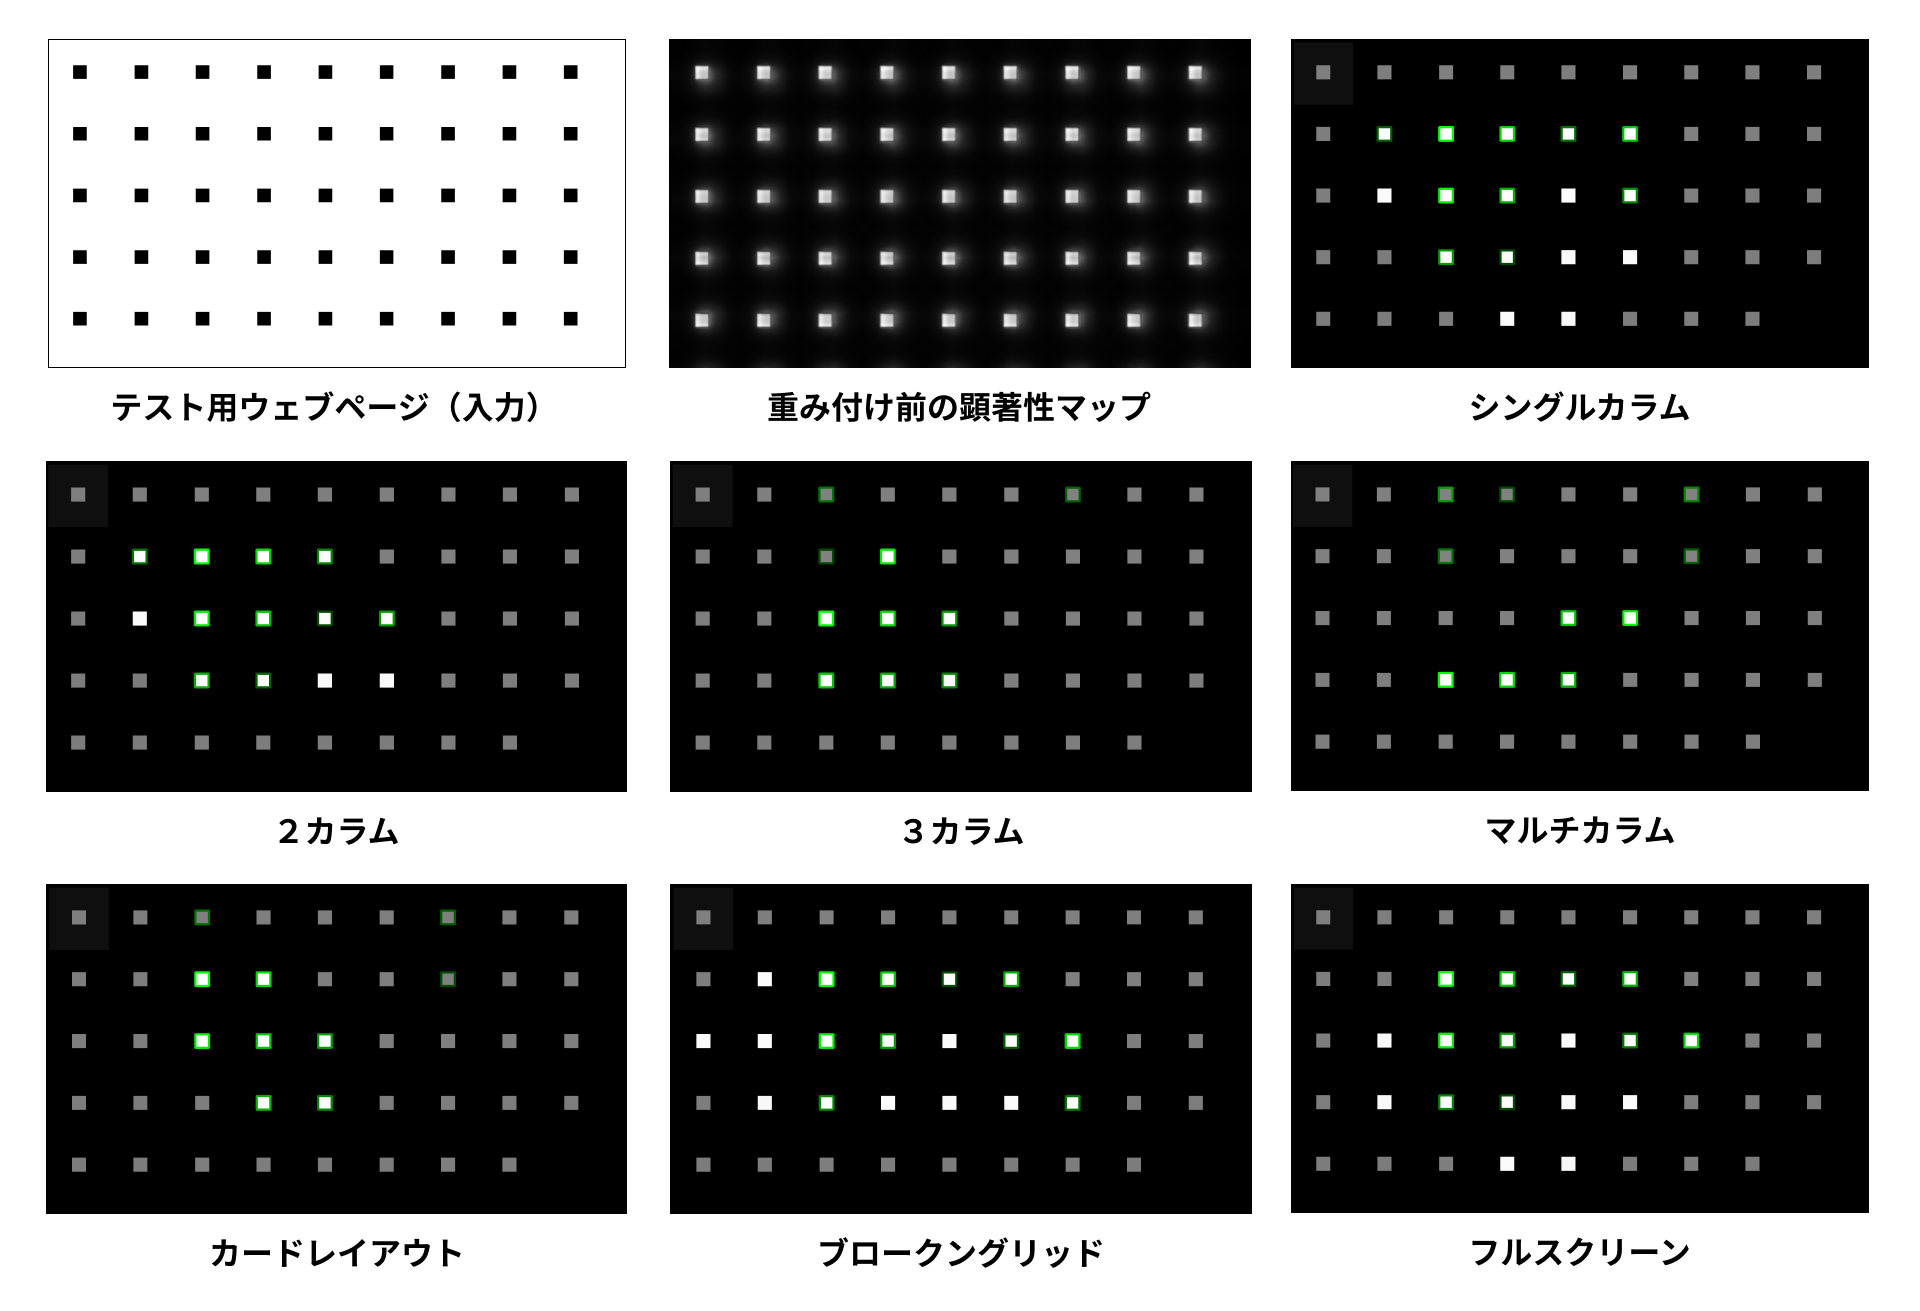
\includegraphics[width=12cm]{figures/06_positionbias.jpg}
    \caption{位置情報による重み付けのシミュレーション}
    \label{fig_positionbias}
\end{figure}


\subsection{顕著領域の視覚化}\label{subsec:system04}
\par ここでは第\ref{subsec:system03}節で計算した要素ごとの顕著度を元に顕著領域の視覚化を行う。本システムでは、顕著度が高い重要領域を要素単位で塗りつぶした顕著領域マップと特に顕著度が高い要素を一つにまとめた集約図の2つの出力を行う。顕著領域の視覚化の流れを図\ref{fig_system04}に示す。

\begin{figure}[H]
    \centering
    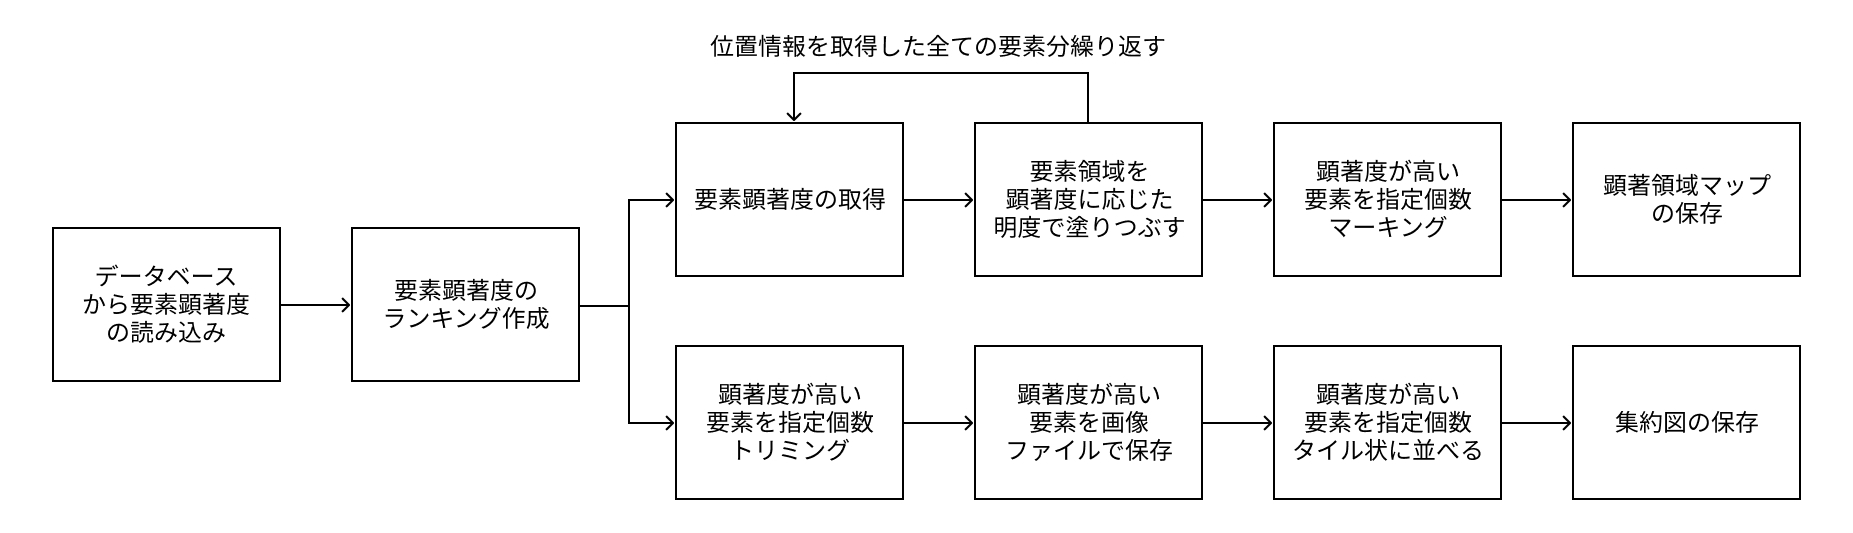
\includegraphics[width=12cm]{figures/06_process04.jpg}
    \caption{顕著領域の視覚化の流れ}
    \label{fig_system04}
\end{figure}

\subsubsection{顕著度ランキングの生成}\label{subsec:system04-1}
\par 顕著領域マップと集約図の生成にあたり、第\ref{subsec:system03}節で計算した顕著度のランキングを作成する。顕著度ランキングの計算アルゴリズムをアルゴリズム\ref{alg:lanking}に示す。まず始めに、第\ref{subsec:system03}節でデータベースに保存した顕著度を顕著度が高い順にソートする。本来であれば、顕著度が高い順にランキングを付ければ良いが、図\ref{fig_system4-rank}に示すように同一要素を内包している他の要素も顕著度が高く評価されてしまう問題が生じる。同じ要素が顕著度ランキングに何度も出現する事は問題である為、一度顕著度が高いと評価した要素を内包する外部の要素をNGリストに格納して顕著度ランキングに入らないように評価する。また、ウェブページの要素の中には装飾等の為に極端に細長い要素など顕著度ランキングに不必要なノイズが存在する。これらの要素を取り除く為にフィルターをかけて極端な形状の要素を取り除いた。

\newpage
\begin{algorithm}[H]
  \small
  \caption{顕著度ランキング}
  \label{alg:lanking}
  \begin{algorithmic}

  \State stag\_list $ \leftarrow $ CSVの読み組み
  \State tag\_list\_num $ \leftarrow $ CSVの行数
  \State salient\_level = [] // 顕著度を格納するリスト
  \State ng\_list = [] // NGリスト
  \State high\_element\_list = [] // 顕著度ランキングを格納するリスト
  \For{$i$ in $range(tag\_list\_num)$}
    \State salient\_level.append(tag\_listのi行目の要素の顕著度)
  \EndFor    
  \State salient\_level\_sort $ \leftarrow $ salient\_levelをソート
  \State salient\_num $ \leftarrow $ 10 //顕著度ランキングを生成する個数
  \State temporal\_num $ \leftarrow $ 1
  \State salient\_num\_first $ \leftarrow $ salient\_num

  \While{while salient\_num $>$ 0}
    \State most\_salient $ \leftarrow $ salient\_level\_sort[tag\_list\_num - temporal\_num]
    \If{(most\_salient in ng\_list) == False}
    \State start\_x, start\_y, end\_x, end\_y $\leftarrow$ CSVのmost\_salient行目から取得
    \State size $\leftarrow$ CSVからmost\_salient行目の要素のwidth $*$ heightを取得
    \If{(end\_x $-$ start\_x)/(end\_y $-$ start\_y) $<$ 10}
    \State high\_element\_list.append(most\_salient)
    \State salient\_num $\leftarrow$ salient\_num - 1
    \For{$i=1$ in $range(tag\_list\_num)$}
    \If{(most\_salient in ng\_list) == False}
    \State r\_start\_x, r\_start\_y, r\_end\_x, r\_end\_y $\leftarrow$ i行目から取得
    \State r\_size $\leftarrow$ CSVからi行目の要素のwidth*heightを取得
    \If{i行目要素とmost\_salient行目要素が内包関係}
    \If{r\_size $-$ size $<$ 200 $or$ size $-$ r\_size $<$ 200}
    \State ng\_list.append(i) //NGリストにi行目要素を格納
    \EndIf
    \EndIf
    \EndIf
    \EndFor 
    \EndIf
    \Else
    \State temporal\_num $\leftarrow$ temporal\_num $+$ 1
    \EndIf
  \EndWhile
  \end{algorithmic}
\end{algorithm}

\begin{figure}[H]
    \centering
    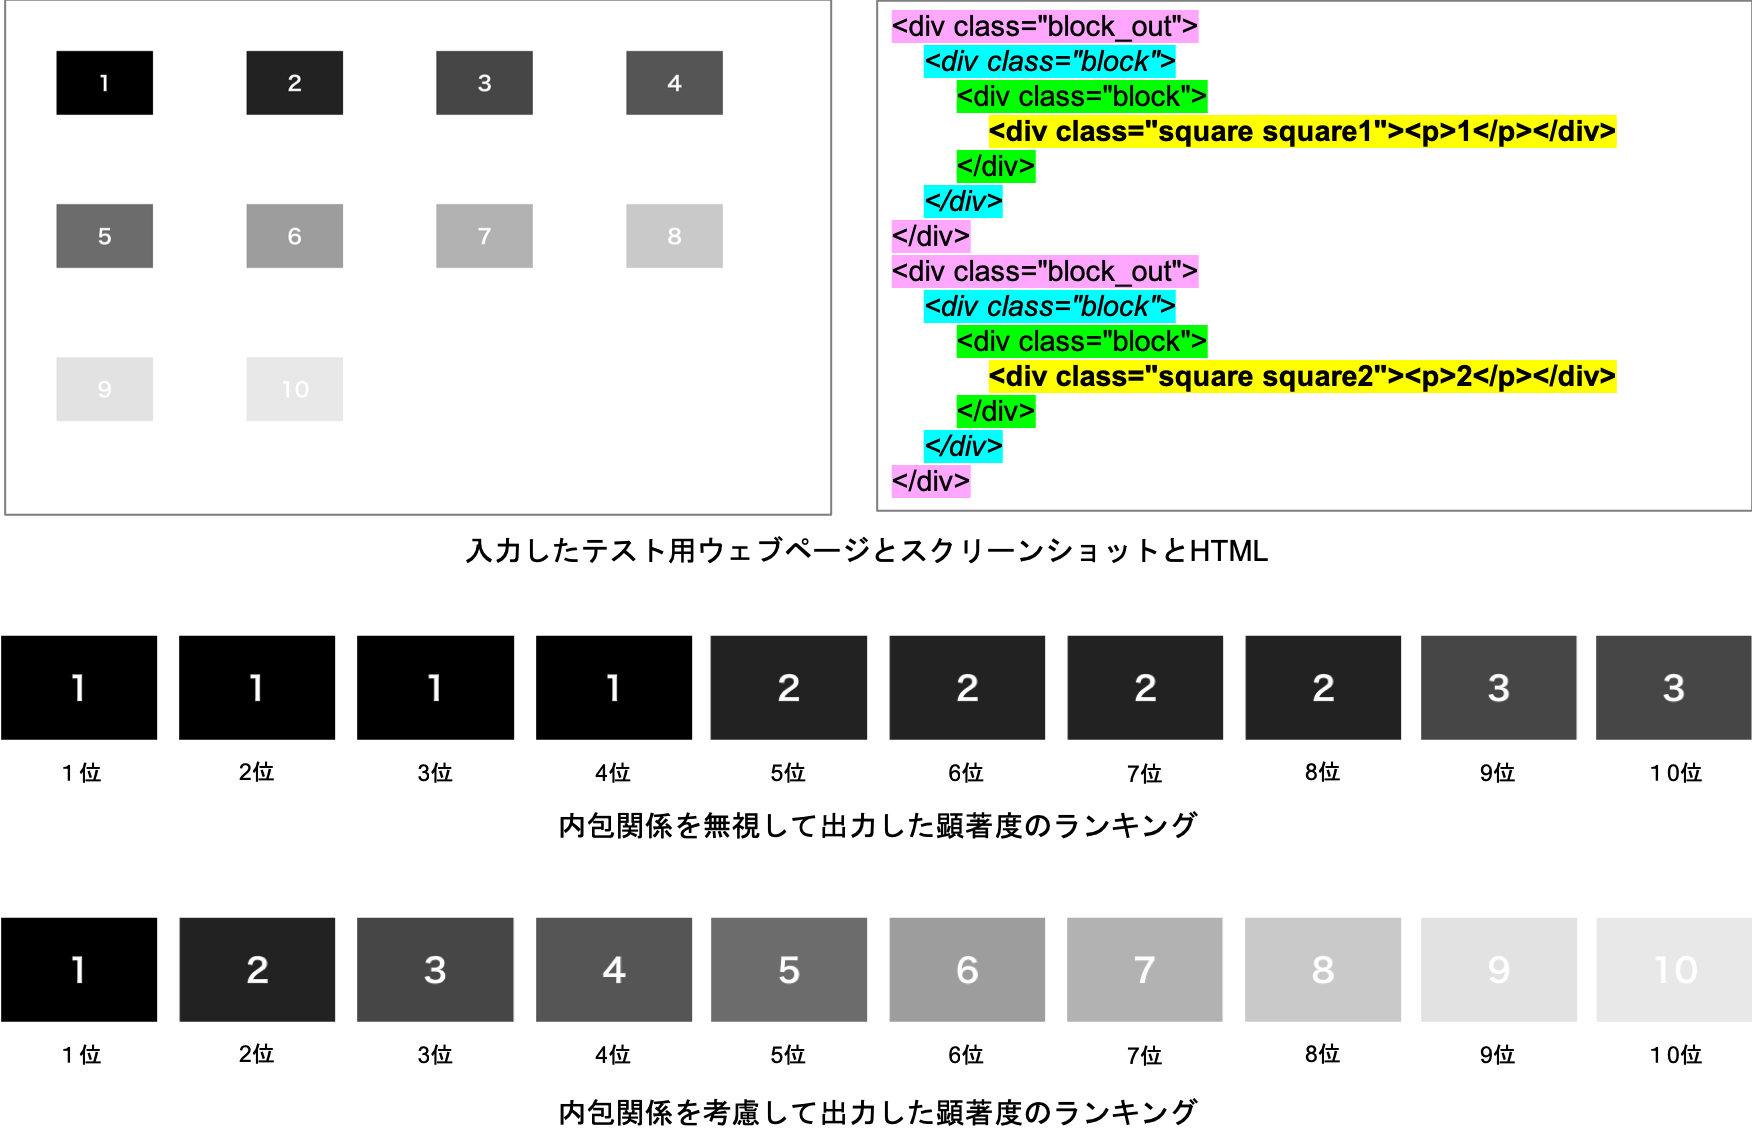
\includegraphics[width=12cm]{figures/06_rank.png}
    \caption{要素の内包関係を考慮した時としない時の顕著度ランキング}
    \label{fig_system4-rank}
\end{figure}

\subsubsection{顕著領域マップの生成}\label{subsec:system04-1}
\par 顕著領域マップの生成方法について説明する。第\ref{subsec:system03}節で計算した各要素の顕著度は上限なしの単精度浮動小数点型で表されている。要素を顕著度に応じた明度で塗りつぶす為にはコンピューター上で表現できる色の濃度の0$\sim$255の範囲内で表現する必要がある。本システムでは最も顕著度の高い要素の明度が$255$になるように顕著そを圧縮して、位置情報を取得した画面上に表示されている全ての要素の領域をこの顕著度を明度とした長方形で塗り潰す。

\par さらに、特に顕著度が高い重要領域を視覚化する為に第\ref{subsec:system04-1}項で作成した顕著度ランキングの指定個数(デフォルトは10個)の要素の外枠を顕著度が高い順に明るい緑色の線で描写する。このことにより、要素の塗りつ潰された明度の微妙な差異を簡単に見分ける事が可能になる。以上の作業を行う事で顕著領域マップの生成を行う。図\ref{fig_output-example}にテスト用ウェブページのURLを入力して生成された顕著領域マップの例を示す。なお、テストページには左図のように大きさが同じ長方形でそれぞれ異なる明度で塗りつぶされた要素が等間隔に並べられたページを作成して使用した。

\subsubsection{集約図の生成}\label{subsec:system04-2}
\par 集約図の生成方法について説明する。第\ref{subsec:system04-1}項で作成した顕著度ランキングを元に顕著度が特に高い指定個数(デフォルトは10個)の要素の領域をスクリーンショットから切り取りタイル状に並べる。本システムでは上段に上位2個を、中段に3位$\sim$5位の3個を、下段には6位$\sim$10位の5個を並べる事で顕著度が高い要素が大きい面積で表示されるようにした。図\ref{fig_output-example}に顕著領域マップの説明と同様のテスト用ウェブページのURLを入力して生成された集約図の例を示す。顕著度が高く目立ちやすい1番の要素から順番にタイル状に並べられてどの要素が注目されやすいのかを一目で確認する事が可能である。

\begin{figure}[H]
  \centering
  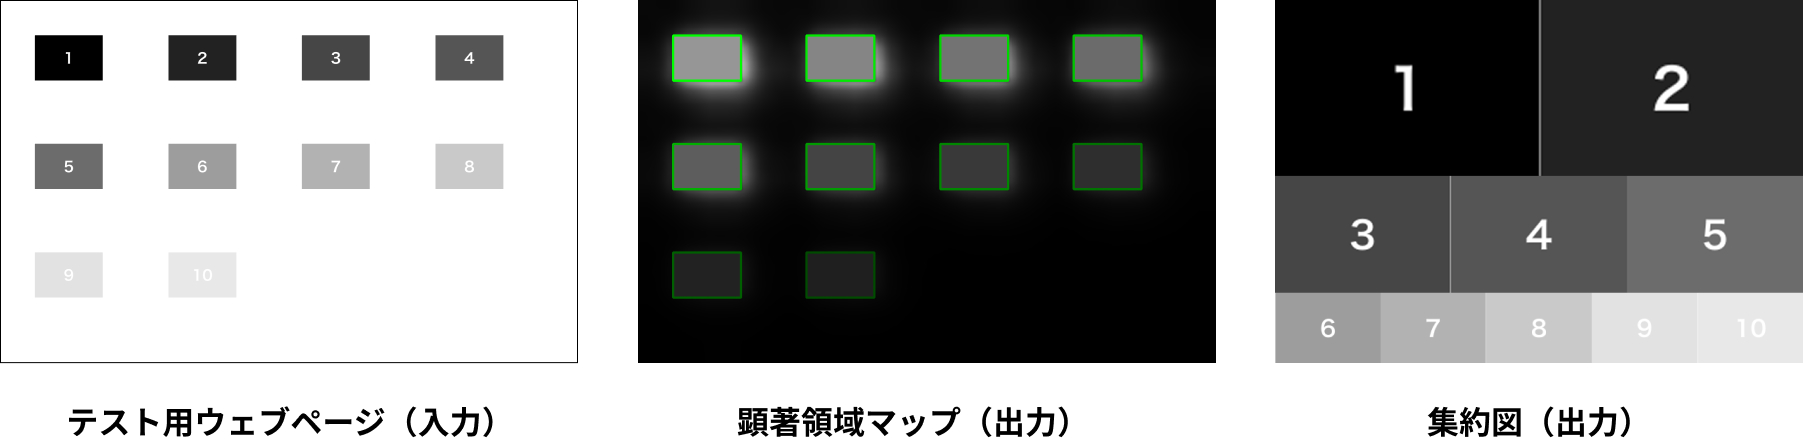
\includegraphics[width=12.5cm]{figures/06_example-output.png}
  \caption{生成される顕著領域マップと集約図の例}
  \label{fig_output-example}
\end{figure}

% 第7章 評価
\newpage
\renewcommand{\baselinestretch}{1.5}
\section{評価}
\renewcommand{\baselinestretch}{1}
\par 本手法を評価する為に要素の顕著度推定の精度に関する評価とウェブページの顕著性マップの可視化を目的として提案した顕著領域マップならびに集約図の認識のしやすさと効果に関する3つの実験を実施した。

\subsection{評価方法}
\subsubsection{要素の顕著度推定精度に関する評価}
\par 1つ目の評価方法では本手法の特徴であるウェブページの要素の顕著度推定精度を測る。第\ref{subsec:webdataset}節で作成したオリジナルのウェブデータセットをランダムに4:1の割合で分析用のページ216個と評価用のページ54個に分類して、54個の評価用ウェブページとその実際の被験者視線データを使用して評価を行う。実験の評価指標としてBylinskiiらの公開プログラム\cite{salMetrics_Bylinskii}のLinear Correlation Coefficient (CC), Area Under the Curve (AUC)とKullback\-Leibler divergence (KL)の3つの顕著性メトリクスを使用した。

\par {\bf AUC (Area Under the Curve)}は顕著性マップ生成モデルに最もよく使用されるメトリクスで横軸を注視点の誤検出率、縦軸を注視点の検出率としたROC曲線の曲線下の面積を計測する評価指標である。$0\sim1$の間で評価され、$0.5$の時にランダムであることを表し$1$に近いほど精度の高い顕著性マップであることを示す。{\bf CC (Linear Correlation Coefficient)}はオリジナルモデルの顕著性マップと実際の被験者の視線データから作成された正解顕著性マップの間の相関係数を計測する評価指標である。CCは$-1\sim1$の間で評価され、$1$に近いほど精度の高い顕著性マップであることを示す。{\bf KL (Kullback\-Leibler divergence)}はオリジナルモデルの顕著性マップと正解顕著性マップの2つの確率分布がどの程度似ているのかを計測する評価指標である。KLは今まで説明した2つのメトリクスとは異なり、2つのマップが同じ確率分布である場合に$0$と評価される為、$0\sim1$の間で評価され、$0$に近いほど精度の高い顕著性マップであることを示す。

\par 評価実験では54個の評価用ウェブページを使用して正解顕著領域マップと我々のオリジナルモデルとプログラムが公開されている関連研究を比較した。評価を行う為に第\ref{subsec:gazedataset}節で取得した被験者の実際の視線データを使用して第\ref{subsec:system04-1}節で説明した手法で正解顕著領域マップを作成した。また、関連研究として公開されている中で評価が高い自然画像向けニューラルネットワーク顕著性マップ生成モデルであるPanらのSalNet\cite{pan2016shallow}とCorniaらのML-NET\cite{mlnet2016}を使用した。さらにオリジナルモデルではIttiらのベーシックな顕著性マップ生成モデル\cite{itti1998model}を使用しているが、顕著性マップ生成モデルを変更することでオリジナルモデルにCorniaらのML-NET\cite{mlnet2016}を組み合わせたものも比較モデルに加える。


\subsubsection{重要領域の認識のしやすさに関する評価}
\par 2つ目の評価方法では最もベーシックなモデルであるIttiらの顕著性マップ生成モデル\cite{itti1998model}と提案手法の顕著領域マップでの重要領域の認識のしやすさについて比較評価した。本実験では20代の19$\sim$25歳の大学生・大学院生10人の日常的にインターネットを使用するインターネットユーザーに対してインタビュー形式で実験を行った。

\par 評価では被験者に顕著性マップの概要について簡単に説明した後に既存の顕著性マップと提案手法の顕著領域マップの例を2つ提示して最後に全7問の表\ref{table:question01}に示す内容のアンケートを実施した。アンケートでは既存の顕著性マップと提案手法の顕著領域マップの重要領域の認識のしやすさの度合いと、どのような点で認識しやすく感じたり認識しにくいと感じるのかを記述式で質問した。また、実験にはJapan Web Design Gallery\cite{japanwebgallery}に掲載されているウェブページの中からランダムに選んだ2つのウェブページ情報を使用した。実験に使用したウェブページの一覧を表\ref{table:webpage-list2}に示す。また、実際に被験者に見せたウェブページと顕著性マップと顕著領域マップの比較を図\ref{fig_experience02}に示す。


\begin{table}[h]
  \caption{重要領域認識実験に使用したウェブページの一覧(2019年1月20日閲覧)}
  \label{table:webpage-list2}
  \centering
  \begingroup
  \renewcommand{\arraystretch}{1.2} % 表の行間の変更
  \small
    \begin{tabular}{llll}
    \hline
    & ページ名 & カテゴリ & URL \\
    \hline \hline
    K & 下関春帆楼 & カフェ・レストラン & https://www.shunpanro.com/ \\
    L & 白洋舎 & クリーニング & http://www.hakuyosha.co.jp/ \\
    \hline
  \end{tabular}
  \endgroup
\end{table}

\begin{figure}[H]
  \centering
  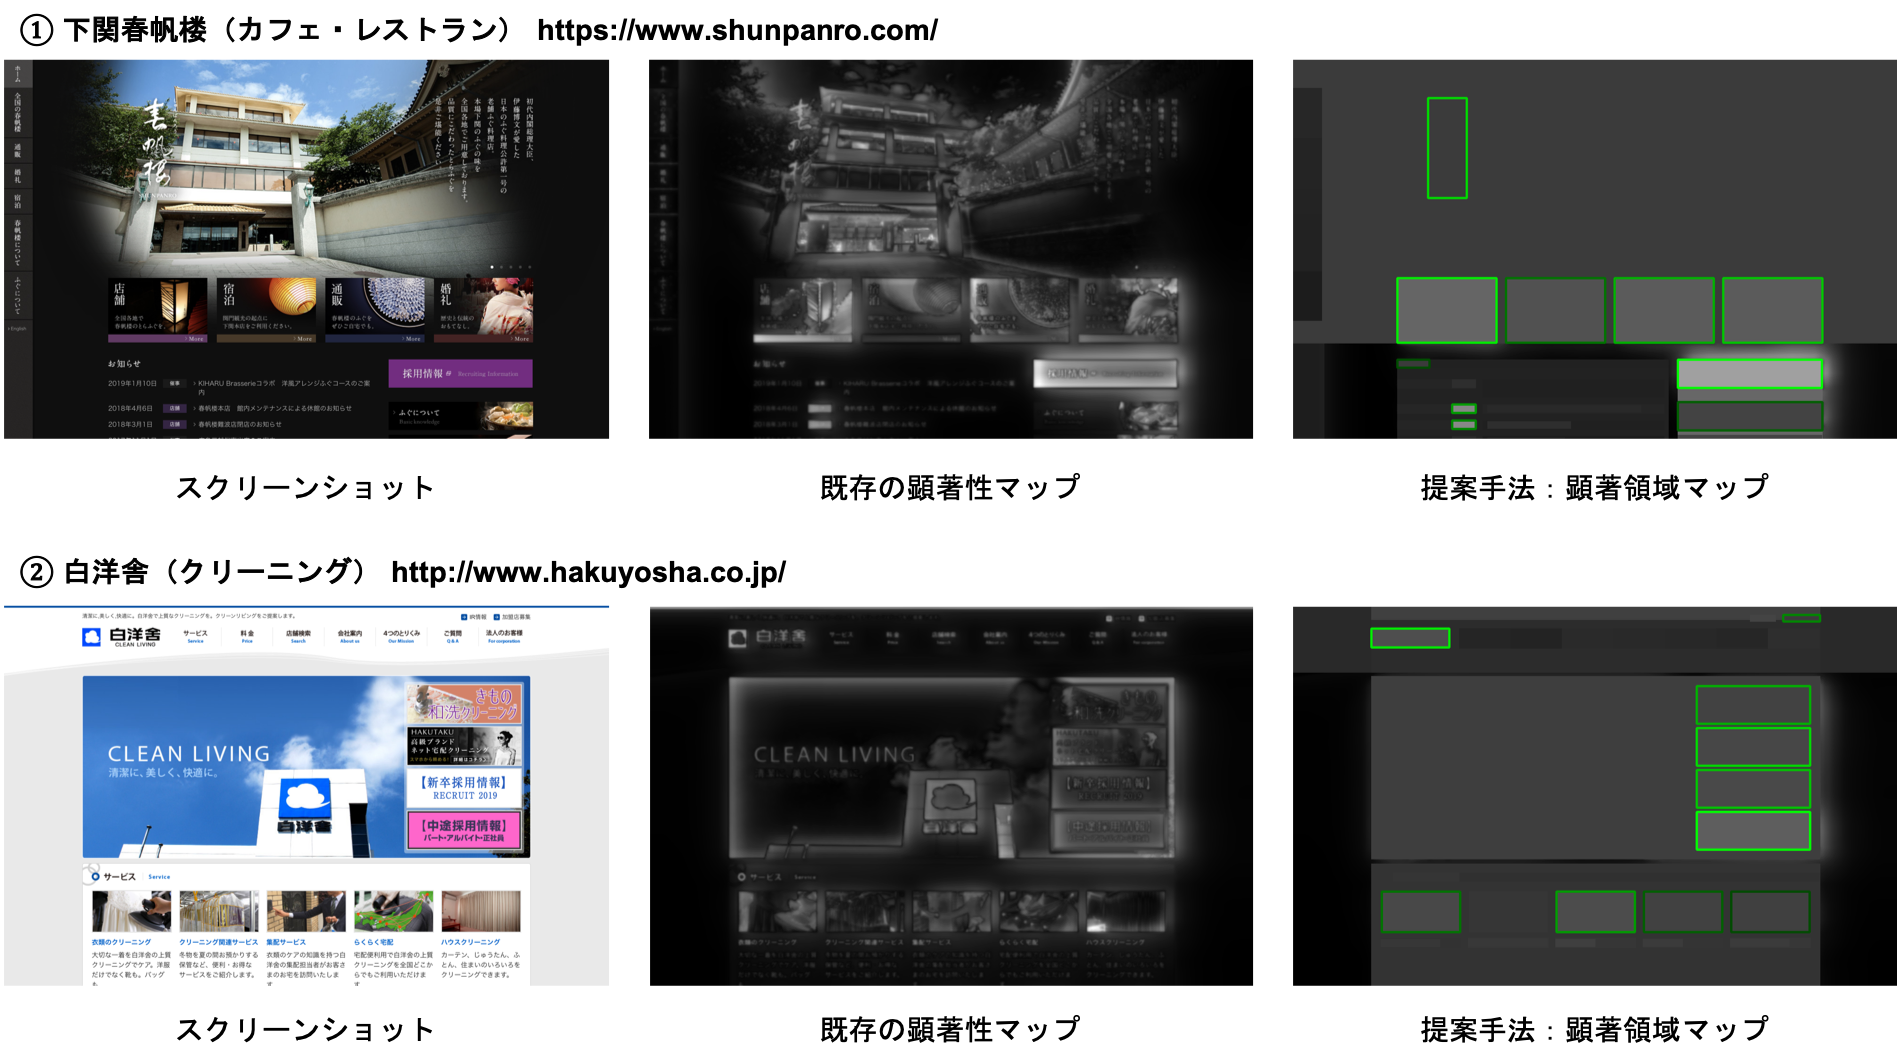
\includegraphics[width=12cm]{figures/07_experience02.png}
  \caption{既存の顕著性マップと提案手法(顕著領域マップ)の比較実験}
  \label{fig_experience02}
\end{figure}

\begin{table}[h]
  \caption{アンケートの質問内容1}
  \label{table:question01}
  \centering
  \begingroup
  \renewcommand{\arraystretch}{1} % 表の行間の変更
  \small
  \begin{tabular}{|l|l|l|l|}
    \hline
    \multicolumn{2}{|c|}{質問内容} & \multicolumn{2}{|c|}{選択肢・記述式} \\ \hline
    & & a & 非常に認識しにくい \\ \cline{3-4}
    & & b & 認識しにくい \\ \cline{3-4}
    Q1 & 既存の顕著性マップは & c & どちらでもない \\ \cline{3-4}
    & 重要領域を認識しやすいと感じるか & d & 認識しやすい \\ \cline{3-4}
    & & e & 非常に認識しやすい \\ \hline
    & & a & 非常に認識しにくい \\ \cline{3-4}
    & & b & 認識しにくい \\ \cline{3-4}
    Q2 & 提案手法の顕著領域マップは & c & どちらでもない \\ \cline{3-4}
    & 重要領域を認識しやすいと感じるか & d & 認識しやすい \\ \cline{3-4}
    & & e & 非常に認識しやすい \\ \hline
    Q3 & 既存の顕著性マップの認識しづらいと感じる点 & \multicolumn{2}{|l|}{記述式} \\ \hline
    Q4 & 既存の顕著性マップの認識しやすいと感じる点 & \multicolumn{2}{|l|}{記述式} \\ \hline
    Q5 & 顕著領域マップの認識しづらいと感じる点 & \multicolumn{2}{|l|}{記述式} \\ \hline
    Q6 & 顕著領域マップの認識しやすいと感じる点 & \multicolumn{2}{|l|}{記述式} \\ \hline
    Q7 & 特定の要素の重要度を調べたい時 & a & 既存の手法 \\ \cline{3-4}
    & どちらの手法が認識しやすいと感じるか  & b & 提案手法 \\ \hline
    \end{tabular}
    \endgroup
\end{table}


\subsubsection{集約図の効果に関する評価}
\par 3つ目の評価方法では特に顕著度が高い重要領域をタイル状に並べてまとめた集約図の効果について評価した。本実験についても20代の19$\sim$25歳の大学生・大学院生10人の日常的にインターネットを使用するインターネットユーザーに対してインタビュー形式で実験を行った。

\par 評価ではまず始めに被験者に図\ref{fig_experience03-2}に示す集約図の例を見せ集約図の意味について簡単に説明したのちに、図\ref{fig_experience03-1}に示す集約図を見てウェブページの内容を予想してもらい、分かる範囲でページ内容を記述式で回答してもらった。また、ウェブページの予測をしてもらった後に表\ref{table:question02}に示す集約図の効果に関する2問の質問に選択式で解答してもらった。なお、アンケートの最後には自由記入形式の感想欄を設けて集約図をみた際の感想などを記述してもらった。集約図の効果検証実験に使用したウェブページを表\ref{table:webpage-list3}に示す。

\begin{table}[h]
    \caption{集約図の効果評価実験に使用したウェブページ(全て2019年1月20日閲覧)}
    \label{table:webpage-list3}
    \centering
    \begingroup
    \renewcommand{\arraystretch}{1.2} % 表の行間の変更
    \small
      \begin{tabular}{llll}
      \hline
      & ページ名 & カテゴリ & URL \\
      \hline \hline
      M & 株式会社エース & コンビニ・スーパー・小売り & https://www.ace-group.co.jp/ \\
      \hline
    \end{tabular}
    \endgroup
\end{table}

\begin{figure}[H]
    \centering
    
\includegraphics[width=10cm]{figures/experience03-2.png}
    \caption{被験者に閲覧してもらった集約図の例}
    \label{fig_experience03-2}
\end{figure}

\begin{figure}[H]
    \centering
    
\includegraphics[width=6cm]{figures/experience03-1.png}
    \caption{ページ内容を予想してもらった集約図(株式会社エースHP)}
    \label{fig_experience03-1}
\end{figure}

\begin{table}[H]
    \caption{アンケートの質問内容2}
    \label{table:question02}
    \centering
    \begingroup
    \renewcommand{\arraystretch}{1} % 表の行間の変更
    \small
    \begin{tabular}{|l|l|l|l|}
        \hline
        \multicolumn{2}{|c|}{質問内容} & \multicolumn{2}{|c|}{選択肢} \\ \hline
        & & a & 全く判断できない \\ \cline{3-4}
        Q8 & 重要領域のみを抽出した集約図を見て & b & 少し判断できる \\ \cline{3-4}
        & ページ内容を判断することはできるか & c & ある程度判断できる \\ \cline{3-4}
        & & d & ほとんど判断できる \\ \hline
        & & a & 全く効果的でない \\ \cline{3-4}
        & 初見のウェブページの内容を一目で & b & あまり効果的でない \\ \cline{3-4}
        Q9 & 確認したい時重要領域を抽出してまとめる & c & どちらでもない \\ \cline{3-4}
        & 手法は効果的だと思うか & d & 効果的である \\ \cline{3-4}
        & & e & 非常に効果的である \\ \hline
        \end{tabular}
        \endgroup
\end{table}

\newpage
\subsection{結果と考察}
\subsubsection{要素の顕著度推定精度に関する評価}\label{subsec:evaluation1}
\par 1つ目の評価方法では被験者の実際の視線から作成した正解顕著領域マップと本手法の顕著領域マップとML-NETを組み合わせたモデルならびに2つの顕著性マップ生成モデルをCCとAUCとKLの3つのメトリクスで評価を行った。なお、正解顕著領域マップと比較対象のモデルについては各モデルのピクセルレベルの顕著性マップを第\ref{subsec:system04-1}節で説明した手順で要素単位の顕著領域マップに変換した上でオリジナルモデルと比較実験を行った。ウェブページデータセットの評価用データ54個の中からいくつか選んでそれぞれのモデルを比較した様子を図\ref{fig_07_eval-models}に示す。正解顕著性マップは1つのウェブページあたり5名の被験者の全ての視線データを加算して作成された実際の顕著性マップで被験者が閲覧した領域を正確に表している。また、正解顕著性マップを元に要素単位の顕著度を計算して各要素を顕著度に応じた明度で塗り潰したものが正解顕著領域マップである。この正解顕著領域マップとオリジナルモデルや比較モデルであるML-NETやSalNetの類似度を検証することで各モデルの精度を計算した。

\par 図\ref{fig_07_eval-models}を見ると各モデルによって顕著領域マップの出力が大きく異なることが確認できる。各ウェブページの要素の明度は顕著度を表しており、明るい要素ほど注目されやすいことを示し暗い要素ほど注目されにくい要素であることを示す。ウェブページによって正解データに近いモデルは異なるが他のモデルと比較して本手法のオリジナルモデルは正解顕著領域マップに近いことが確認できる。

\par 評価用の合計54個全てのウェブページの比較検証を行い各メトリクスの平均を計算した結果を表\ref{fig_07_eval-models}に示す。調査の結果より3個のメトリクスの内、顕著性マップ生成モデルの評価指標として最もよく使われるAUCとKLの2つのメトリクスではオリジナルモデルが最も良いスコアを獲得した。また、CCについてもオリジナルモデルはML-NETに劣るスコアになったものの、オリジナルモデルにML-NETを組み合わせたモデルが最も良いスコアを獲得した。メトリクスの一つであるCCで他のモデルに劣るスコアが計測されたことはCC(Linear Correlation Coefficient)はマップの間の相関係数を計測する評価指標であるため画像間の輝度の差を計算することが原因であると考えられる。隣り合う各要素の顕著度のバランスの精度が高くても全体的に顕著度が低く出力されることで結果的に相関係数が低くなってしまったと考える。しかしながら、全体的にオリジナルモデルは要素の顕著度推定精度は高くウェブページの顕著領域マップを生成するモデルとして最適であると言える。


\begin{figure}[H]
  \centering
  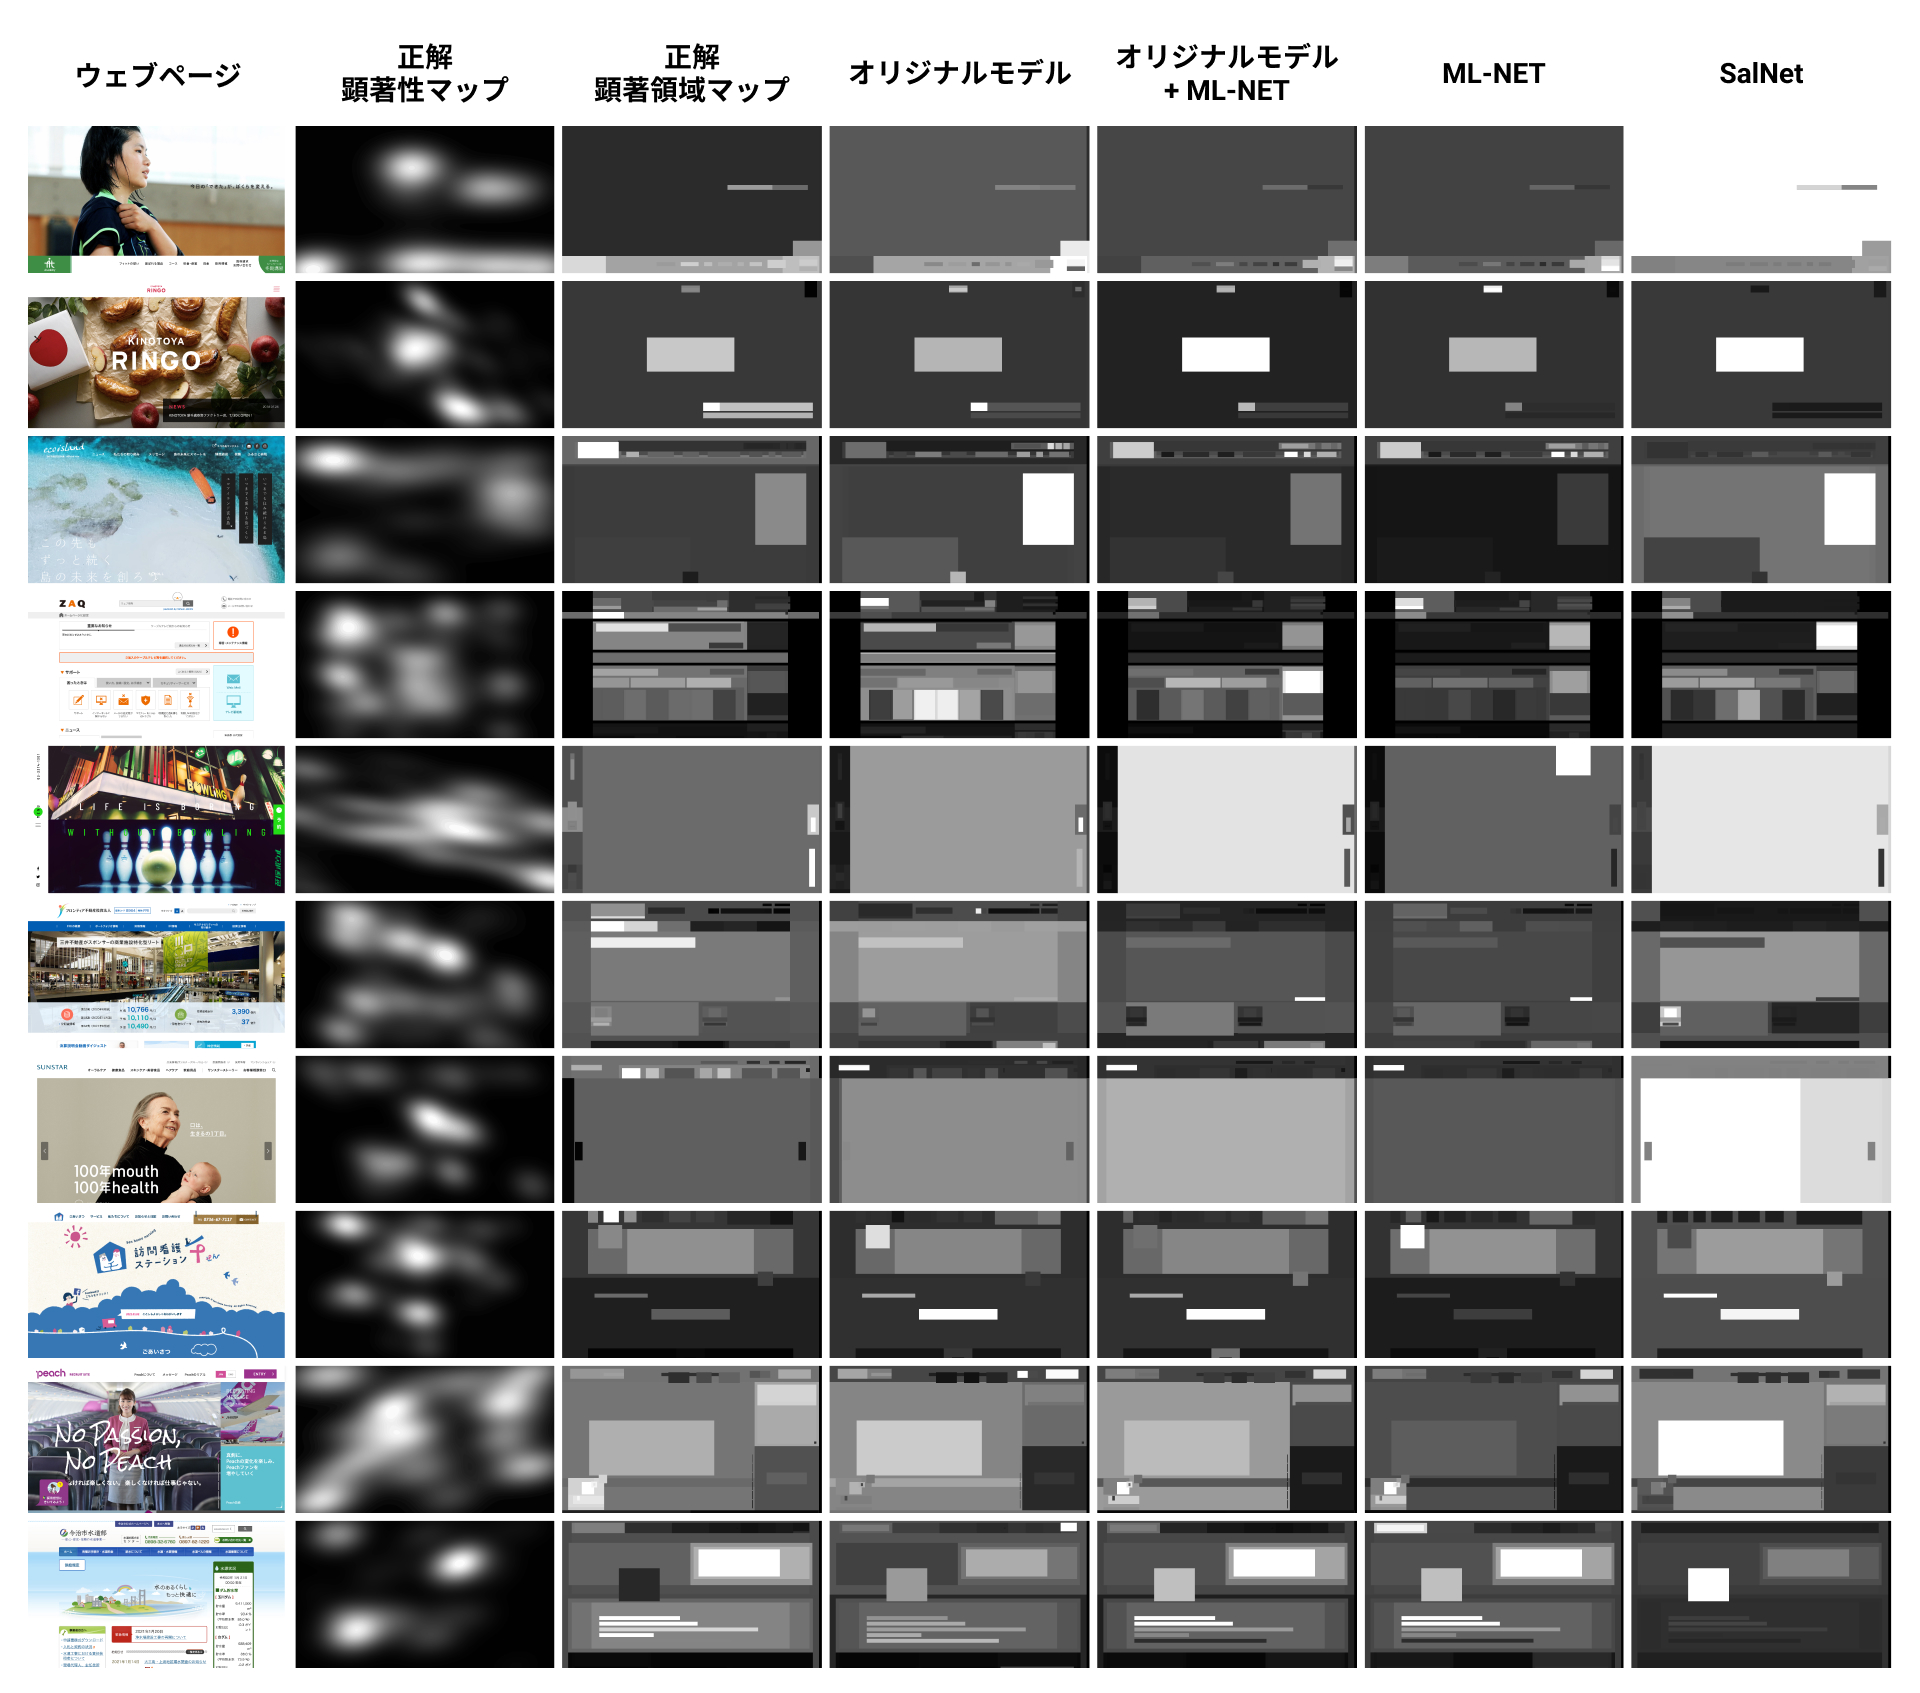
\includegraphics[width=12.5cm]{figures/07_eval-models.jpg}
  \caption{オリジナルモデルと顕著性マップモデルの比較}
  \label{fig_07_eval-models}
\end{figure}

\begin{table}[h]
  \caption{異なるモデル間でのパフォーマンス評価}
  \label{table:webpage-list2}
  \centering
  \begingroup
  \renewcommand{\arraystretch}{1.2} % 表の行間の変更
  \small
   \begin{tabular}{lccc}
    \hline
    & AUC↑ & CC↑ & KL↓ \\
    \hline \hline
    オリジナル & {\bf 0.786118} & 0.53475 & {\bf 0.12348} \\
    オリジナル + ML-NET & 0.743187 & {\bf 0.55167} & 0.13691 \\
    SalNet & 0.662697 & 0.36863 & 0.14679 \\
    ML-NET & 0.742791 & 0.54798 & 0.13777 \\
    \hline
  \end{tabular}
  \endgroup
\end{table}


\subsubsection{重要領域の認識のしやすさに関する評価}
\par 2つ目の評価方法では既存の顕著性マップの一例であるIttiらの顕著性マップ生成モデルと提案手法の顕著領域マップでの重要領域の認識のしやすさについてアンケート形式で評価した。重要領域の認識のしやすさについて質問した2つの質問の評価結果を図\ref{fig_evaluation02-1}に示す。既存の顕著性マップは「認識しやすい」と「認識しにくい」と回答した被験者が4名ずつで、「どちらでもない」と「非常に認識しにくい」と回答した被験者が1名ずつで比較的否定的な意見が目立つ結果となった。一方で提案手法の顕著領域マップでは「非常に認識しやすい」と回答した被験者が4名、「認識しやすい」と回答した被験者が5名、「どちらでもない」と回答した被験者が1名で「認識しにくい」や「非常に認識しにくい」などの否定的な意見は存在しなかった。以上の結果より、手案手法の顕著領域マップは既存の顕著性マップと比較して重要領域の認識という点において明らかに優れている。

\par また、記述式で質問した既存の顕著性マップと提案手法の顕著領域マップのそれぞれの重要領域の認識のしやすさと認識のしにくさに関する問いでは既存の顕著性マップ重要領域の認識のしずらさとして挙げられた「要素の境界が分かりづらい」や「最も顕著度の高い要素がどれなのか顕著の度合いを比較しにくい」などといった意見を提案手法の顕著領域マップで改善できたという肯定的な意見が多かった。しかしながら様々な意見の中には「元のウェブページの様子が見えない為スクリーンショットと照らし合わせる必要がある」や「顕著度ランキングの枠線の濃淡の差が分かりづらい」などといった元のウェブページの様子が全く見えなくなった提案手法の顕著領域マップならではの問題点もいくつか挙げられた。これらの問題点を解決する為に例えば元のウェブページの画像と顕著領域マップを重ね合わせたり簡単に切り替えることが出来るようなGUIを作成したりランキングの枠の隣に番号を付けるなどの顕著領域マップを作成した後の見せ方にも工夫する必要があることが分かった。上記の提案手法の顕著領域マップの認識のしづらさとして挙げられた問題点は今後の改善に生かして行く必要があると考える。

\par さらに、既存の顕著性マップと提案手法の顕著領域マップのどちらの方が特定の要素の重要度を調べたいときに認識しやすいか質問した問いでは被験者10名全員が提案手法の顕著領域マップの方が優れていると回答した。以上の事から提案手法の顕著領域マップは\ref{subsec:evaluation1}で説明した要素の顕著度推定精度と共に重要領域の認識のしやすさも既存の顕著性マップと比較して改善されたと言える。

\begin{figure}[H]
    \centering
    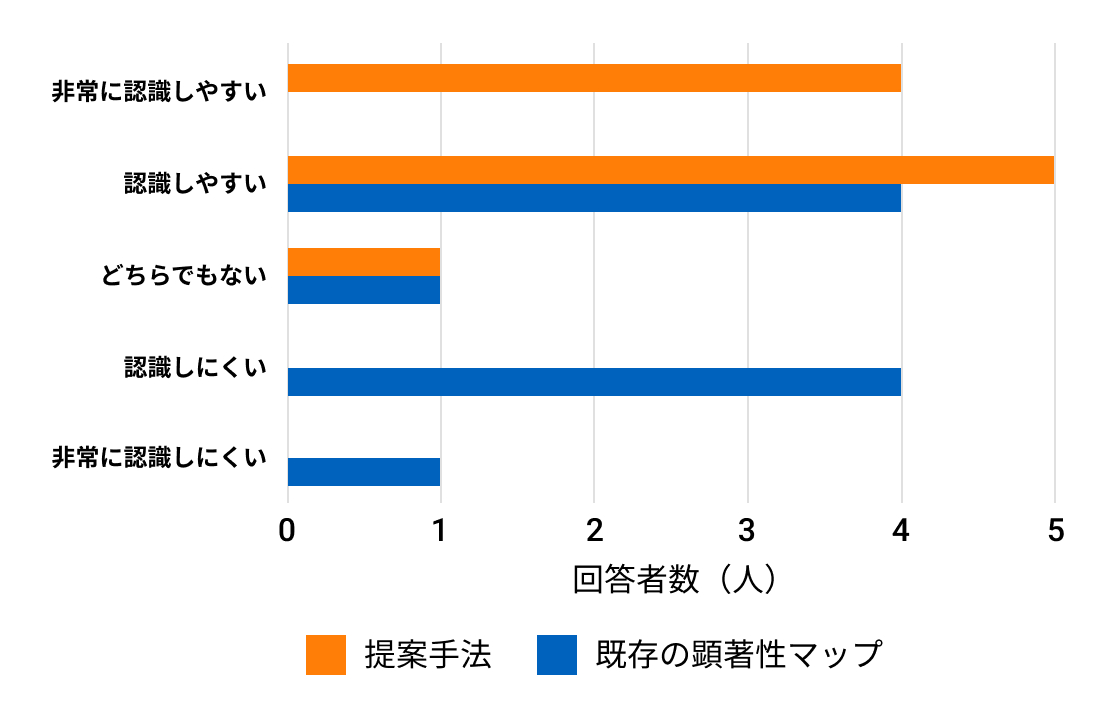
\includegraphics[width=10cm]{figures/07_result01.jpg}
    \caption{顕著領域マップの重要領域の認識のしやすさに関する評価結果}
    \label{fig_evaluation02-1}
\end{figure}

\subsubsection{集約図の効果に関する評価}
\par 3つ目の評価方法ではウェブページの特に顕著度が高い要素をランキング順にタイル状に並べて一枚の画像にまとめた集約図の効果について評価した。集約図の効果を測定する為に図\ref{fig_experience03-1}のように集約図の例を見せてウェブページの内容を予想してもらう問いでは「食品系を取り扱う企業のホームページ」などといったざっくりとしたページ内容は被験者全員が理解することが出来た。しかしながら「関東に展開するスーパーを展開する企業」などのより詳細な内容については理解することが難しい結果となった。提案手法の集約図の目的としてこの図を見ることでユーザーが探している内容がウェブページの内容とマッチしているかどうかを一目で確認できるというものがあるが、難しいということが分かった。

\par 顕著度が高い要素を抽出した集約図を見てウェブページの内容をどの程度判断できるかを質問した結果を表\ref{table:evaluation03-1}に示す。被験者の8名が「ある程度判断できる」で2名が「少し判断できる」と回答しており、ほとんどの被験者が集約図を見ることである程度のページの内容を理解することができるということが分かった。次に初見のウェブページの内容を一目で確認したい時に集約図が効果的だと思うかを質問した結果を表\ref{table:evaluation03-2}に示す。こちらの問いでは6名が「効果的である」と答えた一方で「どちらでもない」や「あまり効果的でない」と回答した被験者が2名ずついた。また「非常に効果的である」と回答した被験者がいなかったことから集約図を閲覧することでウェブページの大枠は理解できるものの細かい内容についてまでは理解できないということが確認できた。集約図のウェブページの内容を一目で確認するという目的については現状では達成できておらず、表示項目を増やしたりレイアウトや見せ方を変更するなどの工夫が必要であることが分かった。

\begin{table}[H]
    \caption{Q8の回答結果}
    \label{table:evaluation03-1}
    \centering
    \begin{tabular}{lc}
      \hline
      選択肢 & 回答数 \\
      \hline \hline
      ある程度判断できる & 8 \\
      ほとんど判断できる & 0 \\
      少し判断できる & 2 \\
      全く判断できない & 0 \\
      \hline
    \end{tabular}
\end{table}

\begin{table}[H]
    \caption{Q9の回答結果}
    \label{table:evaluation03-2}
    \centering
    \begin{tabular}{lc}
      \hline
      選択肢 & 回答数 \\
      \hline \hline
      非常に効果的である & 0 \\
      効果的である & 6 \\
      どちらでもない & 2 \\
      あまり効果的でない & 2 \\
      全く効果的でない & 0 \\
      \hline
    \end{tabular}
\end{table}

% 第8章 おわりに
\newpage
\renewcommand{\baselinestretch}{1.5}
\section{おわりに}
\renewcommand{\baselinestretch}{1}
\par 本研究では、ウェブページのレイアウトに着目して要素単位での顕著度を計測することでウェブページに特化した重要領域の視覚化手法を提案した。まず初めにパブリック上に存在しなかったモダンデザインを含めたウェブページのオリジナル視線データセットを作成した。このデータセットでは合計270個のウェブページを使用して35名の被検者の
視線データを収集した。また、被験者の視線データを分析することでウェブページ固有の視線のバイアスやレイアウトによる傾向などを新たに確認することができた。

\par オリジナルデータセットを用いて取得したウェブページの視線データセットを用いてウェブページ固有の要素に着目して要素単位のレイアウトを考慮した正確な顕著度の推定を行った。さらに要素ごとの顕著度を可視化する為に提案手法である顕著領域マップの生成を行った。提案手法の顕著領域マップの顕著度推定精度は他のニューラルネットワークモデルと比較して高く、重要領域の見やすさについても既存の顕著性マップと比較して認識しやすいことが明らかになりウェブページに最適な顕著度可視化マップであると言える。これによりデザイナーはユーザーがウェブページを閲覧した際にどの要素に注目する可能性が高いのかをウェブページの開発段階で正確に判断する事が可能となる。また、それに合わせて注目してほしい情報を上手に配置することで、その情報にユーザーが注目しやすくなり効率的なユーザーの獲得につながるのではないかと考えられる。

\par さらに、計算された要素単位での顕著度を用いて顕著度のランキングを作成した。このランキングを使用することで特に顕著度が高い要素をタイル状に並べて一つの画像で表した集約図の生成を行なった。集約図についてはウェブページの内容理解面で詳細内容までは理解することが難しいなどの課題が残る結果となった。これらの顕著度推定後の可視化面でより見やすいレイアウトなどの工夫を行うことでウェブページの内容理解支援ツールとして改善できると考える。\\

\par 本研究の今後の課題は以下の通りである。

\begin{itemize}
  \item 顕著領域マップの見せ方の改善
  \par ~~本手法では要素単位で顕著度に応じた明度で塗り潰すことで顕著領域マップの生成を行った。しかしながら、被験者の意見の中に元のウェブページと照らし合わせる必要があるなどの視認性の問題が挙げられた。これらの問題を解決する為にGUI上で元のウェブページとボタンで切り替えるなどの見せ方の改善を行うことでより使いやすく分析しやすいものに改善できると考えている\\

  \item 集約図の見せ方の改善
  \par ~~本手法で被験者から最も否定的な意見が多かったのが顕著度の高い重要領域をまとめた集約図の見せ方についてである。ウェブページの内容理解支援ツールを目的として集約図を提案したが、ページ内容の大枠程度しか理解できずあまり効果的でないという意見が目立った。これらを解決する為、集約図のレイアウトや表示する要素数の変更などを行いウェブページの内容を理解しやすい物へと改善したいと考える。また、過去に研究発表した「ワードクラウドのグラデーション描写による多次元化」\cite{inagaki2018}の技術と組み合わせる事で画像だけでなくウェブページのテキストも合わせて分析した手法も可能か検討したいと考えている。
  \\
\end{itemize}
% % 第2章 ウェブページの構造
\newpage
\renewcommand{\baselinestretch}{1.5} % 行間の倍率指定
\section{ウェブページの構造}\label{sec:scraping}
\renewcommand{\baselinestretch}{1} % 行間の倍率指定
\par 近年PHPやRubyなど様々なプログラミング言語によりウェブページやウェブアプリケーションは開発されているが、最終的にはHTML(Hyper Text Markup Language)と呼ばれるマークアップ言語\cite{mozilla_html}を動的に出力することでウェブブラウザ上にウェブページを表示している。つまり、HTMLを分析することでウェブページの構造が分かるということだ。それらの構造を解析する事で様々な情報を取得する方法としてウェブスクレイピング技術がある。
\subsection{ウェブスクレイピングとは}
\par サーバーサイドのプログラムを使用することで外部サーバーにアクセスしてウェブサイト上から必要な情報を取得することをウェブスクレイピングという\cite{ntt_scraping}。似たような技術としてAPIが存在するがAPIはサービス提供者側が技術者向けに情報提供する機能のことで、ウェブスクレイピングとは異なる。通常はウェブページのタイトルや株価などの可変数値を取得する目的で使用されることが多いが、本研究ではスクリーンショットの取得やウェブページの構造解析の為にHTMLと各タグ要素の位置情報を取得する為に使用する。

\subsection{ライブラリ}
\par ウェブスクレイピングを簡単に出来るように汎用性のあるプログラムを再利用可能なように集めたライブラリが数多く存在する。ここでは本研究で使用したSelenium WebDriver\cite{selenium}とBeautiful Soup\cite{beautifulsoup}の2つのライブラリを説明する。

\begin{itemize}
    \item Selenium WebDriver
    \par ~~Selenium WebDriverはウェブアプリケーションの自動テストツールとして開発され、ウェブブラウザの拡張機能を使用する事でJavaやPython等のプログラムでブラウザの自動操作を行う事が可能である。本研究では、PythonでSelenium WebDriverを使用する事でスクリーンショットやHTMLの取得のほか画像等の要素の位置とサイズを取得する目的で使用した。 \\

    \item Beautiful Soup
    \par ~~Beautiful SoupはSelenium WebDriverとは異なりPython用のライブラリで、取得したHTMLからタグを抽出したり必要な情報を取得したりする事が可能である。本研究では、Selenium WebDriverを用いて取得したHTMLを解析しやすいように加工する目的でBeautiful Soupを使用した。 \\
\end{itemize}


% 謝辞
\newpage
\renewcommand{\baselinestretch}{1.5}
\section*{謝辞}
\par 本研究を勧めるに当たり、御助言、御協力を頂いた早稲田大学基幹理工学研究科情報理工・情報通信専攻の深澤良彰教授に深く感謝致します。また、3年間に渡るご指導をして頂いた東京女子大学現代教養学部心理・コミュニケーション専攻の白銀純子准教授、神奈川工科大学情報学部情報ネットワーク・コミュニケーション学科の岩田一准教授に深く感謝致します。
\addcontentsline{toc}{section}{謝辞}

% 参考文献
\newpage
\bibliographystyle{junsrt}
\bibliography{thesis}
\addcontentsline{toc}{section}{参考文献}

% 研究業績
\newpage
\section*{研究業績}
\par 稲垣有哉, 深澤良彰, “ワードクラウドのグラデーション描写による多次元化”, 2018年電子情報通信学会 基礎・境界ソサイエティ/NOLTAソサエティ大会, 金沢大学角間キャンパス, 石川県金沢市, 2018年9月11~14日.\\
\par 稲垣有哉, 岩田一, 白銀純子, 深澤良彰, “ウェブページの構造と顕著性マップの組み合わせによる重要領域の確認支援手法”, 2019年情報処理学会, 全国大会, 福岡大学七隈キャンパス, 福岡県福岡市, 2019年3月14~16日.\\
\par 稲垣有哉, 岩田一, 白銀純子, 深澤良彰, “ウェブページの構造と顕著性マップの組み合わせによる重要領域の視覚化手法”, ARG 第14回Webインテリジェンスとインタラクション研究会, 兵庫県立大学神戸商科キャンパス, 兵庫県神戸市, 2019年6月28~29日.\\
\par Yuya Inagaki, Hajime Iwata, Junko Shirogane, Yoshiaki Fukazawa, “Visualization Method of Important Regions by Combination of Webpage Structures and Saliency Maps”, 15th International Conference on Software Technologies, Conference Paper, Online, July 2020.\\


\addcontentsline{toc}{section}{研究業績}

\end{document}
